% Paquets généraux
\documentclass[a4paper,12pt,titlepage]{article}
\usepackage[T1]{fontenc}
\usepackage[utf8]{inputenc}
\usepackage[french]{babel}
\usepackage[gen]{eurosym}
%\usepackage[dvips]{graphicx}
\usepackage{fancyhdr}
\usepackage{pdfpages} 
\usepackage{multido}
\usepackage{hyperref}
%\usepackage{textcomp}
%\usepackage{aeguill}
\usepackage{schemabloc}
\usepackage[bitstream-charter]{mathdesign}

\newcommand{\id}{54}
\newcommand{\nom}{Liaisons mécaniques}
\newcommand{\sequence}{04}
\newcommand{\num}{01}
\newcommand{\type}{TP}
\newcommand{\descrip}{Modélisation d'un solide. Comportement des liaisons mécaniques. Modéliser les mécanismes du laboratoire par un schéma cinématique, paramétré.}
\newcommand{\competences}{A3-C4: Analyse d'architecture et de comportement \\ &  Mod1-C1: Isolement d'un solide ou d'un système de solides \\ &  Mod2-C10-1: Modèle de solide indéformable \\ &  Mod2-C11: Modélisation géométrique et cinématique des mouvements entre solides indéformables \\ &  Mod2-C12: Modélisation cinématique des liaisons entre solides \\ &  Mod2-C15: Modélisation des actions mécaniques \\ &  Rés-C6: Utilisation d'un solveur ou d'un logiciel multi physique \\ &  Com1-C1: Différents descripteurs introduits dans le programme \\ &  Com2-C4: Outils de communication}
\newcommand{\nbcomp}{9}
\newcommand{\systemes}{Plateforme Stewart}
\newcommand{\systemessansaccent}{Plateforme Stewart}
\newcommand{\ilot}{2}
\newcommand{\ilotstr}{02}
\newcommand{\dossierilot}{\detokenize{Ilot_02 Plateforme Stewart}}
\newcommand{\imageun}{Plateforme}

\newcommand{\urlsysteme}{\href{https://www.costadoat.fr/systeme/57}{Ressources système}}
\newcommand{\matlabsimscape}{\href{https://github.com/Costadoat/Sciences-Ingenieur/raw/master/Systemes/Plateforme Stewart/Plateforme_Stewart_Simscape.zip}{Modèle Simscape}}
\newcommand{\solidworks}{\href{https://github.com/Costadoat/Sciences-Ingenieur/raw/master/Systemes/Plateforme Stewart/Plateforme_Stewart_Solidworks.zip}{Modèle Solidworks}}
\newcommand{\edrawings}{\href{https://github.com/Costadoat/Sciences-Ingenieur/raw/master/Systemes/Plateforme Stewart/Plateforme_Stewart.EASM}{Modèle eDrawings}}
\newcommand{\test}{Stewart_param1}
\newcommand{\testi}{Stewart_param2}
\newcommand{\testii}{Stewart_param3}
\newcommand{\testiii}{Stewart_param4}
\newcommand{\testiiii}{Stewart_euler}

\newcommand{\auteurun}{Renaud Costadoat}
\newcommand{\auteurdeux}{Françoise Puig}
\newcommand{\institute}{Lycée Dorian}


\usepackage{color}
\usepackage{xcolor}
\usepackage{colortbl}
\usepackage{helvet}
\renewcommand{\familydefault}{\sfdefault}
\usepackage{amsfonts}
\usepackage{amsmath}
%\usepackage{xspace}
\usepackage{varioref}
\usepackage{tabularx}
%\usepackage{floatflt}
\usepackage{graphics}
\usepackage{wrapfig}
\usepackage{textcomp}
\usepackage{tikz}
\usepackage{wrapfig}
\usepackage{gensymb}
\usepackage[european]{circuitikz}
\usetikzlibrary{babel}
\usepackage{ifthen}
\usepackage{cancel}
\usepackage{etoolbox}
\usepackage{multirow}
%\usepackage{boxedminipage}
\definecolor{gris25}{gray}{0.75}
\definecolor{bleu}{RGB}{18,33,98}
\definecolor{bleuf}{RGB}{42,94,171}
\definecolor{bleuc}{RGB}{231,239,247}
\definecolor{rougef}{RGB}{185,18,27}
\definecolor{rougec}{RGB}{255,188,204}%255,230,231
\definecolor{vertf}{RGB}{103,126,82}
\definecolor{vertc}{RGB}{220,255,191}
\definecolor{forestgreen}{rgb}{0.13,0.54,0.13}
\definecolor{blcr}{rgb}{0.59,0.69,0.84}
\definecolor{blfr}{rgb}{0.32,0.51,0.75}
\definecolor{orfr}{rgb}{0.90,0.42,0.15}
\definecolor{orcr}{rgb}{0.90,0.65,0.50}
\definecolor{orangef}{rgb}{0.659,0.269,0.072}
\definecolor{orange}{rgb}{0.58,0.35,0.063}
\definecolor{orangec}{rgb}{0.43,0.32,0.25}
\definecolor{rcorrect}{rgb}{0.6,0,0}
\definecolor{sequence}{rgb}{0.75,0.75,0.75}
\definecolor{competences}{rgb}{0.61,0.73,0.35}
\definecolor{grisf}{HTML}{222222}
\definecolor{grisc}{HTML}{636363}
\definecolor{normal}{HTML}{4087c4}
\definecolor{info}{HTML}{5bc0de}
\definecolor{success}{RGB}{92,184,92}
\definecolor{warning}{RGB}{240,173,78}
\definecolor{danger}{RGB}{217,83,79}
\hypersetup{                    % parametrage des hyperliens
    colorlinks=true,                % colorise les liens
    breaklinks=true,                % permet les retours à la ligne pour les liens trop longs
    urlcolor= blfr,                 % couleur des hyperliens
    linkcolor= orange,                % couleur des liens internes aux documents (index, figures, tableaux, equations,...)
    citecolor= forestgreen                % couleur des liens vers les references bibliographiques
    }

% Mise en page
\pagestyle{fancy}

\setlength{\hoffset}{-18pt}

\setlength{\oddsidemargin}{0pt} 	% Marge gauche sur pages impaires
\setlength{\evensidemargin}{0pt} 	% Marge gauche sur pages paires
\setlength{\marginparwidth}{00pt} 	% Largeur de note dans la marge
\setlength{\headwidth}{481pt} 	 	% Largeur de la zone de tête (17cm)
\setlength{\textwidth}{481pt} 	 	% Largeur de la zone de texte (17cm)
\setlength{\voffset}{-18pt} 		% Bon pour DOS
\setlength{\marginparsep}{7pt}	 	% Séparation de la marge
\setlength{\topmargin}{-30pt} 		% Pas de marge en haut
\setlength{\headheight}{35pt} 		% Haut de page
\setlength{\headsep}{20pt} 		% Entre le haut de page et le texte
\setlength{\footskip}{30pt} 		% Bas de page + séparation
\setlength{\textheight}{700pt} 		% Hauteur de l'icone zone de texte (25cm)
\setlength\fboxrule{1 pt}
\renewcommand{\baselinestretch}{1}
\setcounter{tocdepth}{1}
\newcommand{\cadre}[2]
{\fbox{
  \begin{minipage}{#1\linewidth}
   \begin{center}
    #2\\
   \end{center}
  \end{minipage}
 }
}

\newcounter{num_quest} \setcounter{num_quest}{0}
\newcounter{num_rep} \setcounter{num_rep}{0}
\newcounter{num_cor} \setcounter{num_cor}{0}

\newcommand{\question}[1]{\refstepcounter{num_quest}\par
~\ \\ \parbox[t][][t]{0.15\linewidth}{\textbf{Question \arabic{num_quest}}}\parbox[t][][t]{0.93\linewidth}{#1}\par
}


\newcommand{\reponse}[1]
{\refstepcounter{num_rep}
\noindent
\rule{\linewidth}{.5pt}
\textbf{Question \arabic{num_rep}:}
\multido{\i=1+1}{#1}{~\ \\}
}

\newcommand{\cor}
{\refstepcounter{num_cor}
\noindent
\rule{\linewidth}{.5pt}
\textbf{Question \arabic{num_cor}:} \\
}

\newcommand{\titre}[1]
{\begin{center}
\cadre{0.8}{\huge #1} 
\end{center}
}


% En tête et pied de page
\fancypagestyle{normal}{%
  \fancyhf{}
\lhead{\nom}
\rhead{
\includegraphics[width=2cm]{../../img/logo}\hspace{2pt}}
\ifdef{\auteurdeux}{\lfoot{\auteurun,\auteurdeux}}{\lfoot{\auteurun}}
\cfoot{Page \thepage}}

\fancypagestyle{correction}{%
  \fancyhf{}
  \lhead{\colorbox{danger}{\begin{minipage}{0.65\paperwidth} \textcolor{white}{\textbf{Correction}} \end{minipage}} }
  \rhead{
\includegraphics[width=2cm]{../../img/logo}}
  \ifdef{\auteurdeux}{\lfoot{\auteurun,\auteurdeux}}{\lfoot{\auteurun}}
  \rfoot{\colorbox{danger}{\begin{minipage}{0.5\paperwidth} \begin{flushright}\textcolor{white}{\textbf{Correction}}\end{flushright} \end{minipage}} }}

\renewcommand{\footrulewidth}{0.4pt}

\usepackage{eso-pic}
\newcommand{\BackgroundPic}{%
\put(0,0){%
\parbox[b][\paperheight]{\paperwidth}{%
\vfill
\begin{center}
\hspace{0.5cm}\vspace{0.5cm}

\includegraphics[width=\paperwidth,height=\paperheight,%
keepaspectratio]{../../img/fond3}%
\end{center}
\vfill
}}}

\newcommand{\BackgroundPicdeux}{%
\put(25,-30){%
\parbox[b][\paperheight]{\paperwidth}{%
\vfill
\begin{center}
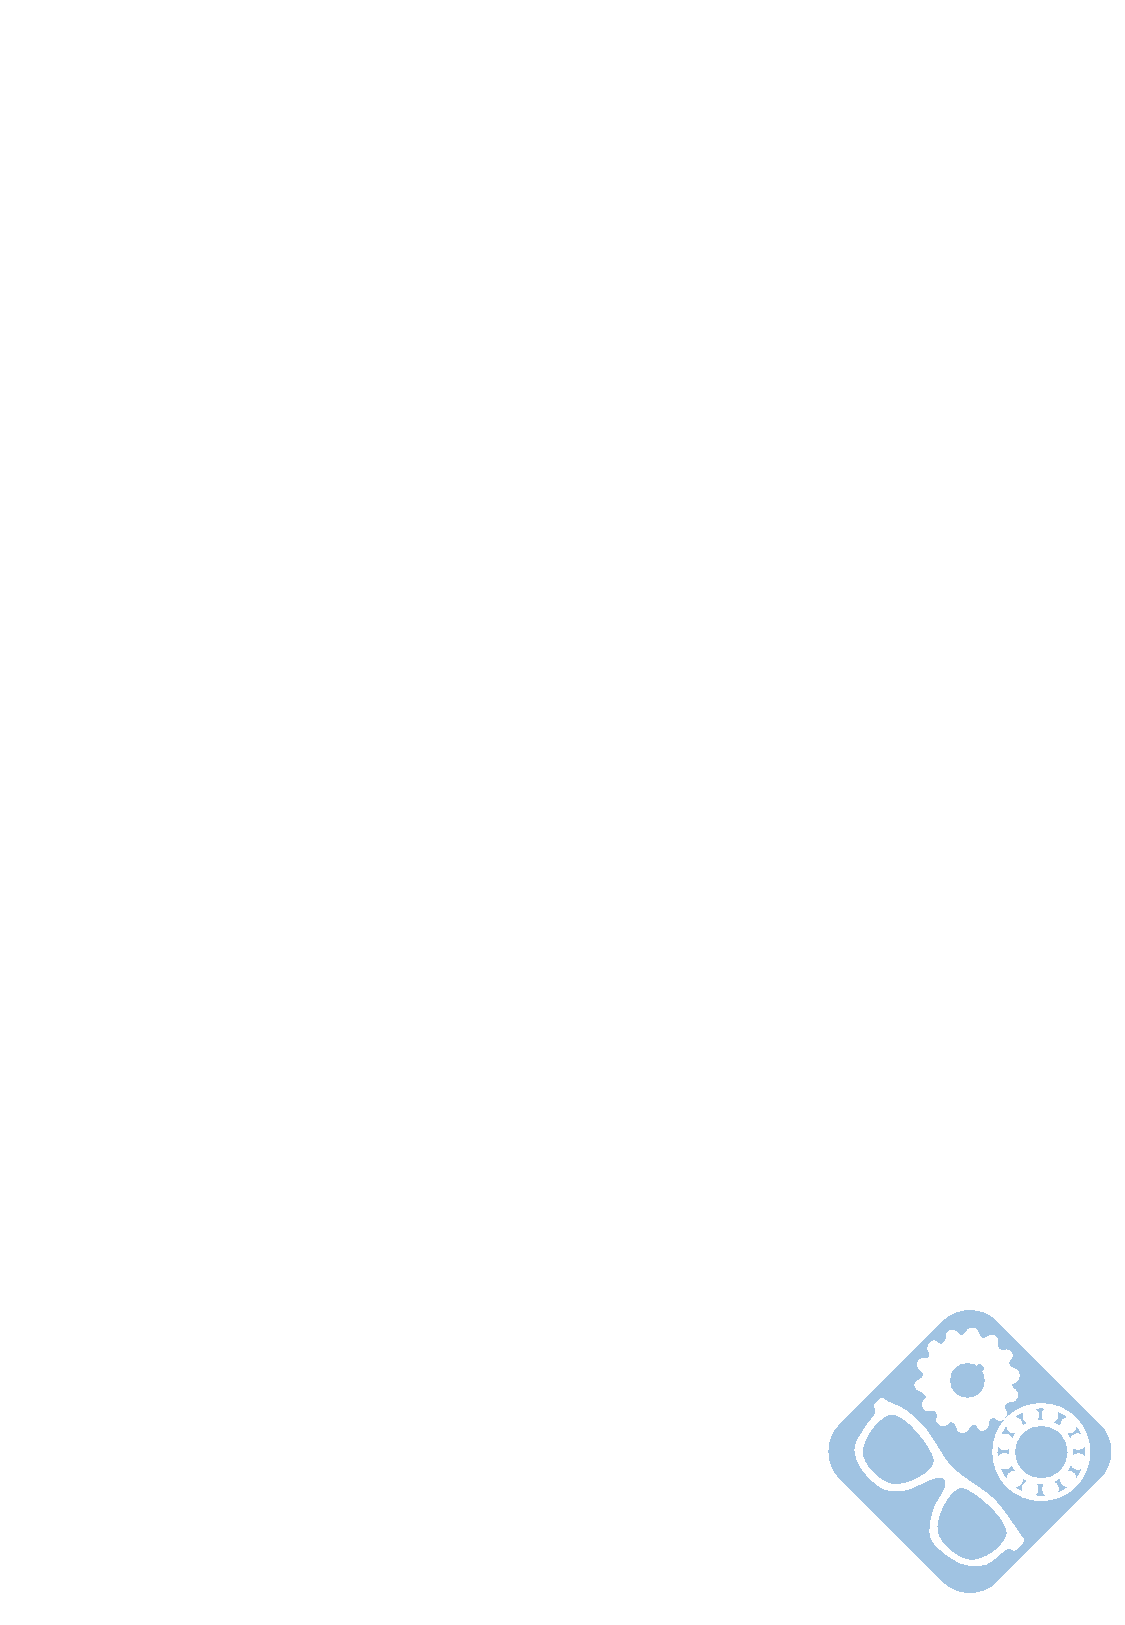
\includegraphics[width=\paperwidth,height=\paperheight,%
keepaspectratio]{../../img/fond4}%
\end{center}
\vfill
}}}

\begin{document}

\pagestyle{empty}

\vspace*{-3\baselineskip}

\AddToShipoutPicture*{\BackgroundPic}

\ifdef{\auteurdeux}{\begin{tabular}{>{\columncolor{gray!00}}m{.3\linewidth} m{.3\linewidth} >{\columncolor{gray!00}}m{.3\linewidth}}
Séquence : \sequence &  \multirow{3}{*}{\hspace{1cm}
\includegraphics[height=1.5cm]{../../img/logo}} &  \begin{flushright} \multirow{4}{*}{\hspace{1cm}
\includegraphics[height=4cm]{img/qrcode}}\end{flushright}\\
Document : \type\num \\
 \institute \\
 \auteurun\\
 \auteurdeux
\end{tabular}}{\begin{tabular}{>{\columncolor{gray!00}}m{.3\linewidth} m{.3\linewidth} >{\columncolor{gray!00}}m{.3\linewidth}}
Séquence : \sequence &  \multirow{3}{*}{\hspace{1cm}
\includegraphics[height=1.5cm]{../../img/logo}} &  \begin{flushright} \multirow{4}{*}{\hspace{1cm}
\includegraphics[height=4cm]{img/qrcode}}\end{flushright}\\
Document : \type\num \\
 \institute \\
 \auteurun
\end{tabular}}

\vspace{1cm}

\ifdef{\prive}{\begin{center}\colorbox{danger}{\Huge{Avec Correction}}\end{center}}{}

\begin{center}\huge{\nom}\end{center}

\vspace{2cm}

\ifdef{\imagedeux}{\begin{minipage}{0.49\linewidth}}{}
\begin{center}\includegraphics[height=5cm]{/home/renaud/Documents/Renaud/GitHub/django_education/systemes/\imageun}\end{center}
\ifdef{\imagedeux}{\end{minipage}\hfill
\begin{minipage}{0.49\linewidth}
\begin{center}\includegraphics[height=5cm]{/home/renaud/Documents/Renaud/GitHub/django_education/systemes/\imagedeux}\end{center}
\end{minipage}}{}

\vspace{5cm}


\begin{tabular}{p{.15\linewidth} >{\columncolor{white}}p{.8\linewidth}}
    \rowcolor{gray!20}
    Référence & S\sequence\ - \type\num \\
    Compétences & \competences \\
 	\rowcolor{gray!20}
    Description & \descrip \\
    Système & \systemes
  \end{tabular}

\newpage

\AddToShipoutPicture{\BackgroundPicdeux}

\pagestyle{normal}

\section{Moteur à explosion}

\subsection{Mise en situation}

\begin{figure}[htbp]
\begin{minipage}[c]{.4\linewidth}
\begin{center}
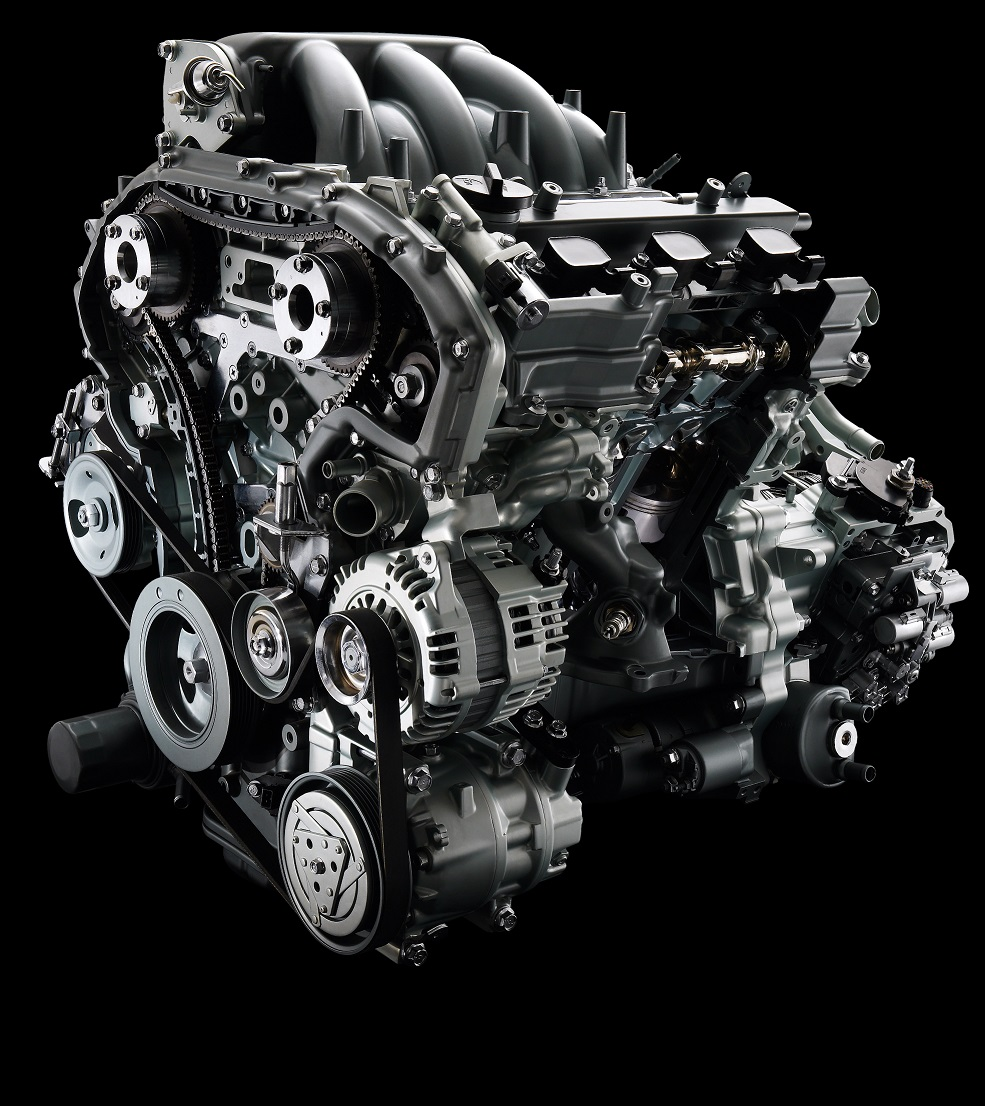
\includegraphics[width=\linewidth]{img/moteur_laguna.jpg}
\caption{Moteur de Renault Laguna}
\label{fig:image8}
\end{center}
\end{minipage}
\hfill
\begin{minipage}[c]{.55\linewidth}
Le moteur à explosion est un type de moteur à combustion interne, il est principalement utilisé pour la propulsion des véhicules de transport (avion à hélice, automobile, moto, camion, bateau), ainsi que pour une multitude d'outils mobiles (tronçonneuse, tondeuse à gazon) ainsi que pour des installations fixes (groupe électrogène, pompe).

Le terme moteur à explosion, consacré par l'usage est impropre car il ne rend pas compte de tous les phénomènes se produisant dans ces moteurs, pour lesquels la dénomination à combustion interne est nettement plus adéquate.
\end{minipage}
\end{figure}

\subsection{Présentation du système}

Le cycle de fonctionnement se décompose de manière analytique en quatre temps ou phases. Le mouvement du piston est initié par la combustion (augmentation rapide de la température et donc de la pression des gaz) d'un mélange de carburant et d'air (comburant) qui a lieu durant le temps moteur. C'est le seul temps produisant de l'énergie ; les trois autres temps en consomment mais le rendent possible.

Le piston se déplace pendant le démarrage grâce à une source d'énergie externe (souvent un démarreur ou lanceur : un moteur électrique est couplé temporairement au vilebrequin) jusqu'à ce qu'au moins un temps moteur produise une force capable d'assurer les trois autres temps avant le prochain temps moteur. Le moteur fonctionne dès lors seul et produit un couple sur son arbre de sortie.

Voici une description des cycles successifs d'un moteur à quatre temps :

\begin{itemize}
 \item admission d'un mélange air et de carburant vaporisé, présent dans le conduit d'admission, mélange préparé par divers composants (carburateur ou système d'injection indirecte) : ouverture de la soupape d'admission et descente du piston, ce dernier aspire ainsi ce mélange dans le cylindre à une pression de -0,1 à -0,3 bar ;
 \item compression du mélange : fermeture de la soupape d'admission, puis remontée du piston qui comprime le mélange jusqu'à 30 bars et 400 à 500°C dans la chambre de combustion ;
 \item combustion et détente aux environs du point mort haut : moment auquel le piston atteint son point culminant et auquel la compression est au maximum ; la bougie d'allumage, connectée à un générateur d'électricité haute tension, produit une étincelle ; la combustion rapide qui s'ensuit constitue le temps moteur ; les gaz chauds à une pression de 40 à 60 bars repoussent le piston, initiant le mouvement ;
 \item échappement : ouverture de la soupape d'échappement et remontée du piston qui chasse les gaz brûlés détendus dans le collecteur d'échappement.
\end{itemize}

Et un nouveau cycle commence en 1.

\begin{figure}[htbp]
\begin{center}
 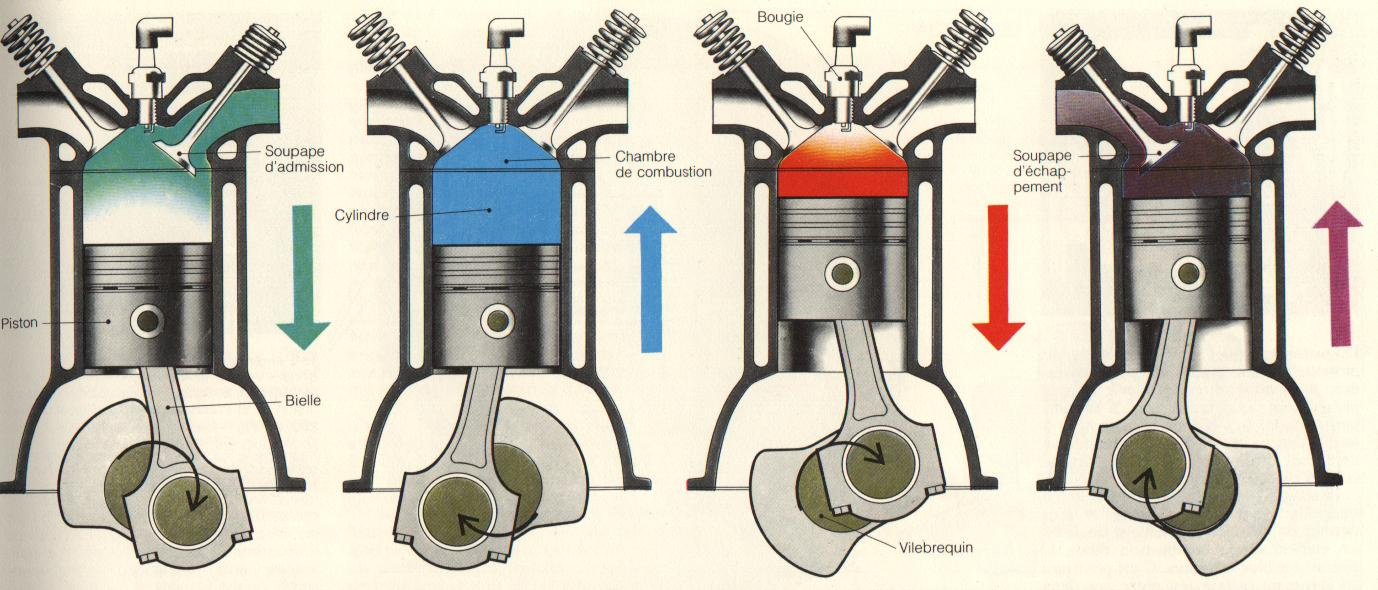
\includegraphics[width=\linewidth]{img/cycles.jpg}
\caption{Cycle de Beau de Rochas}
\label{fig:image9}
\end{center}
\end{figure}

\subsection{Fermeture géométrique}

\paragraph{Question 1:} Représentez le mécanisme du moteur à l'aide d'un schéma cinématique et le paramétrer en y incluant les centres des liaisons ainsi que les repères des pièces.

\paragraph{Question 2:} Déterminer la fermeture géométrique qui donne la position du piston en fonction de la position angulaire du vilebrequin.

\subsection{Fermeture cinématique}

\paragraph{Question 3:} Déterminer les vitesses suivantes:
\begin{itemize}
 \item vitesse du vilebrequin par rapport au bâti, au centre de l'excentrique,
 \item vitesse de la bielle par rapport au bâti, au centre de l'excentrique,
 \item vitesse de la bielle par rapport au bâti, au centre de la liaison entre la bielle et le piston,
 \item vitesse du piston par rapport au bâti, au centre de la liaison entre la bielle et le piston.
 \end{itemize}

\paragraph{Question 4:} A partir d'une loi de composition des vitesses, en déduire la vitesse de déplacement du piston en fonction de la vitesse de rotation du vilebrequin.

\paragraph{Question 5:} Calculer l'accélération du piston par rapport au bâti, au centre de la liaison entre la bielle et le piston.

\newpage

\section{Décocheuse industrielle (E3A MP 2011)}

\subsection{Contexte}

Pour obtenir des pièces de forme complexes (souvent creuses) comme par exemple les carters moteurs pour automobile, le procédé de moulage au sable est souvent utilisé. Un alliage liquide est coulé dans une empreinte de moulage. Cette empreinte de moulage est obtenue par assemblage de deux (ou plus) parties de moule, avec l'ajout dans certains cas de noyaux en sable. Après solidification, la pièce brute peut être extraite du moule. Une des difficultés consiste ensuite à extraire les noyaux de sable présents dans les parties creuses de la pièce moulée.

\begin{center}
	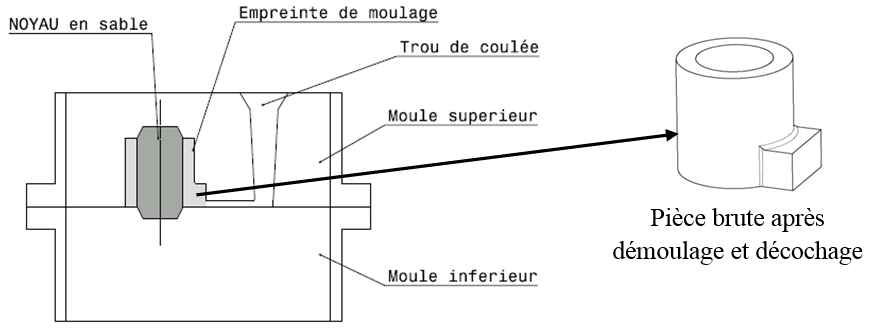
\includegraphics[width=0.7\linewidth]{img/04}
\end{center}

\subsection{Rôle de la décocheuse industrielle}

Une machine de traitement des carters est dans ce cas mise en \oe uvre : une décocheuse. Par une action de secouage (vibration) et de martelage (coups donnés sur la pièce), les noyaux en sables se désagrègent et le sable restant dans la pièce est évacué par gravité.

\begin{center}
	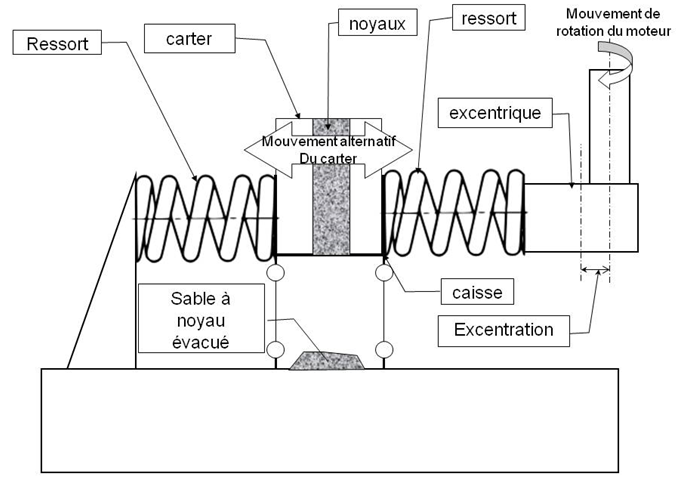
\includegraphics[width=0.7\linewidth]{img/05}
\end{center}

\begin{minipage}{0.55\linewidth}
La décocheuse entraine le carter en vibration pour évacuer le sable des noyaux restant dans ses cavités. Pour cela, le carter à traiter est mis en place dans une caisse. Un moteur entraine un excentrique d'excentration 2mm.

Ce mouvement est amplifié à l'aide de 2 ressorts placés de part et d'autre de l'ensemble caisse + carter pour obtenir	un mouvement amplifié d'amplitude 40mm, ce qui permet l'évacuation du sable des noyaux. Ce dernier est ensuite récupéré en dessous de la caisse.
\end{minipage}\hfill
\begin{minipage}{0.55\linewidth}
\begin{center}
	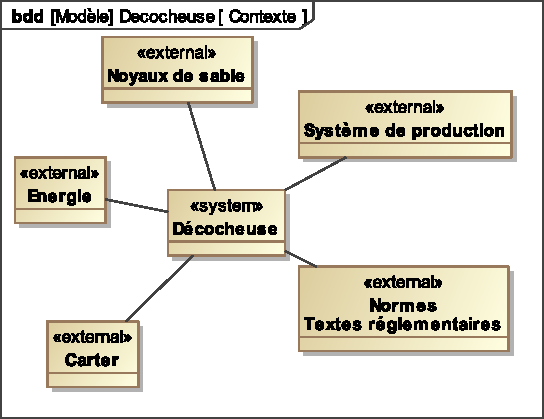
\includegraphics[width=0.7\linewidth]{img/Decocheuse_Contexte}
\end{center}
\end{minipage}

\vspace{0.5cm}

\begin{minipage}{0.59\linewidth}
\begin{center}
	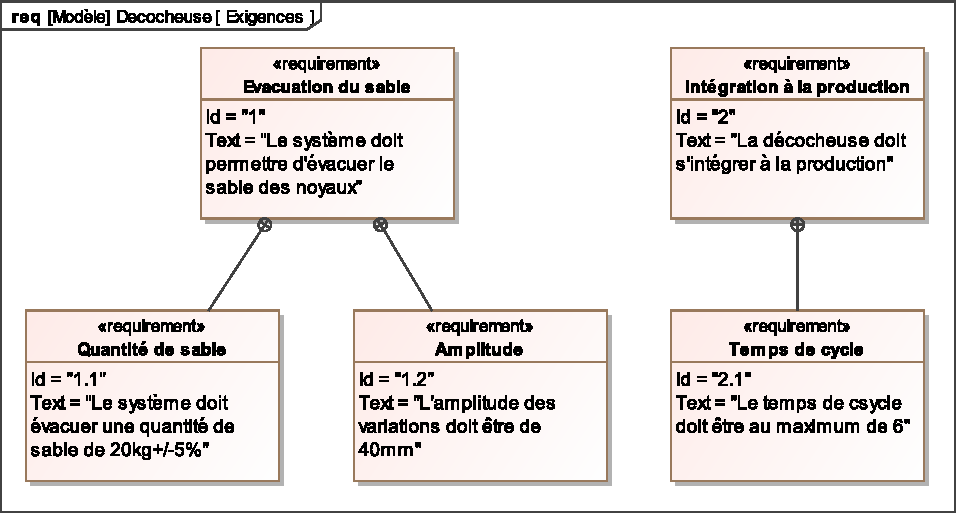
\includegraphics[width=0.9\linewidth]{img/Decocheuse_Exigences}
\end{center}
\end{minipage}\hfill
\begin{minipage}{0.4\linewidth}
Une entreprise souhaite implanter ce type de machine sur sa ligne d'obtention de carters bruts pour réduire le temps de traitement de ses pièces.\begin{center}
	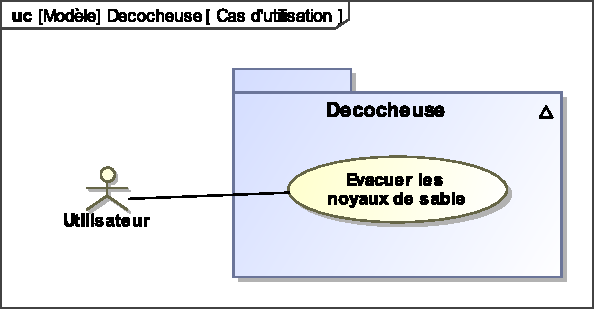
\includegraphics[width=0.9\linewidth]{img/Decocheuse_Cas_utilisation}
\end{center}
\end{minipage}

\vspace{0.5cm}

L'étude suivante va consister à valider le niveau d'amplitude des vibrations de l'ensemble caisse + carter moteur.Pour y arriver, un premier travail portant sur l'étude du mouvement de cet ensemble est demandé. Ce travail préliminaire permet de construire un modèle mathématique représentatif du comportement du système. Ce modèle de connaissance permet alors d'évaluer les performances du système.

\subsection{Evacuer les noyaux de sable}

Dans le cas étudié ici, l'ensemble carter (repère 1) + caisse a une masse de 125 kg au début du cycle (avec le sable) et 105 kg à la fin du cycle. La durée complète du cycle est de 61 secondes. On supposera que, tout au long du cycle, la quantité de sable évacuée est une fonction affine du temps.

\paragraph{Question 1:} Tracer l'évolution temporelle de la masse de l'ensemble (caisse + carter + sable) au cours du cycle et indiquer les valeurs maximales et minimales de la masse. Donner la masse de sable perdu au cours du cycle, notée $M_S$.

On s'intéresse maintenant à la modélisation de la liaison entre la caisse et le bâti. Pour ce faire, des précisions quant aux mouvements relatifs des pièces mises en jeu sont à extraire du schéma cinématique du système.

\begin{center}
	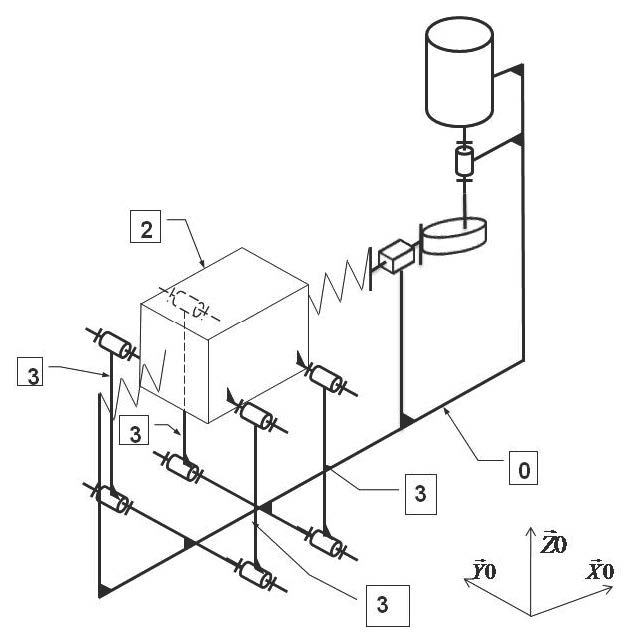
\includegraphics[width=0.7\linewidth]{img/Decocheuse_cin}
\end{center}

Les quatre biellettes (repère 3) sont en liaison pivot d'axe ($Bi,\overrightarrow{Y_0}$) avec la caisse (repère 2) et en liaison pivot d'axe ($Ci,\overrightarrow{Y_0}$) avec le bâti (repère 0).

\begin{center}
	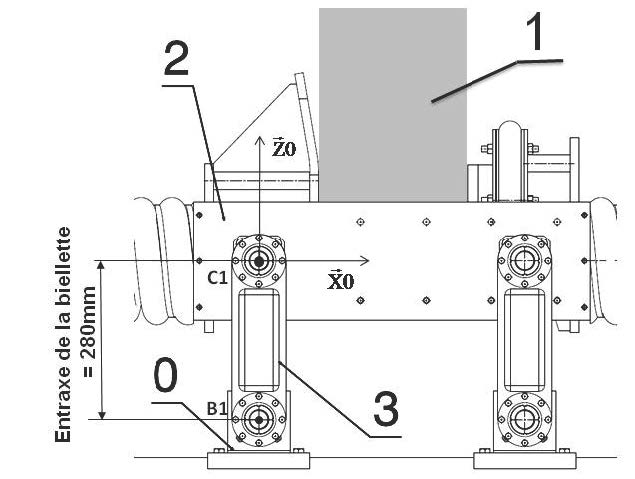
\includegraphics[width=0.7\linewidth]{img/Decocheuse_struc}
\end{center}

L'entraxe de la biellette est de $280 mm$.


\paragraph{Question 2:} Indiquer la nature du mouvement de la caisse (repère 2) par rapport au bâti (repère 0).

\paragraph{Question 3:} Faire un schéma faisant apparaître la trajectoire du point $C_1$ dans son mouvement par rapport au bâti (0). On rappelle que $C_1$ est le centre de la liaison pivot caisse (repère 2) / biellette (repère 3). Indiquer la course du point $C_1$ selon $\overrightarrow{X_0}$ sur votre schéma.

\paragraph{Question 4:} Calculer la valeur du déplacement du point $C_1$ sur l'axe $\overrightarrow{Z_0}$ pour un déplacement variant de -20 mm à +20 mm sur l'axe $\overrightarrow{X_0}$. On donne $\sqrt{14^2-1}=13,96$.

\paragraph{Question 5:} Calculer le ratio de la valeur du déplacement du point $C_1$ sur l'axe $\overrightarrow{Z_0}$ sur la valeur du déplacement sur l'axe $\overrightarrow{X_0}$.

Le ratio calculé à la question 5 montre que le déplacement sur l'axe $\overrightarrow{Z_0}$ est très faible devant celui sur l'axe $\overrightarrow{X_0}$, ce qui permet de modéliser la liaison entre l'ensemble caisse + carter et le bâti par une liaison glissière de direction $\overrightarrow{X_0}$.

La liaison entre la caisse et le bâti étant traitée, on s'intéresse maintenant à la modélisation du générateur de vibration : le système excentrique. Pour cette étude, nous considérons que la bielle (repère 7) est en liaison glissière de direction $\overrightarrow{X_0}$ par rapport au bâti. La liaison entre l'excentrique et la bielle est considérée comme ponctuelle.

\begin{center}
	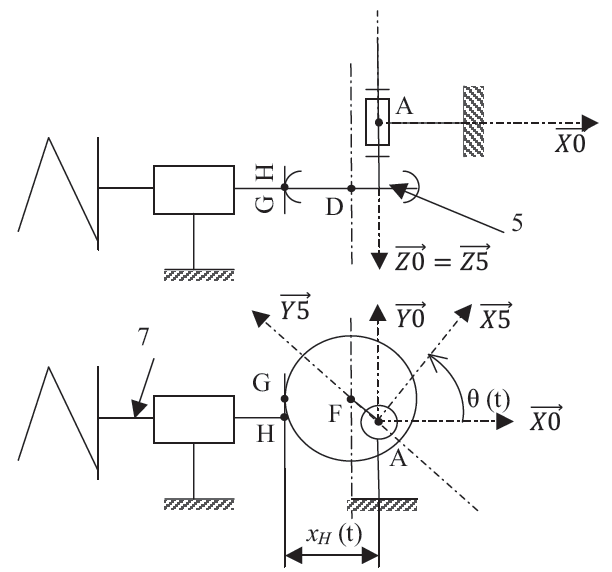
\includegraphics[width=0.55\linewidth]{img/Decocheuse_cin2}
\end{center}

Notation:
\begin{itemize}
 \item $e$ valeur de l'excentration = $AF$,
 \item $R$ rayon de l'excentrique = $FG$,
 \item $\theta$ angle de rotation de l'excentrique
 \item $x_H=\overrightarrow{HA}.\overrightarrow{x_0}$,
 \item $\overrightarrow{\Omega_{5/R_0}}=\dot{\theta}(t).\overrightarrow{z_0}$ avec $\dot{\theta}(t)=\frac{d\theta}{dt}$.
\end{itemize} 

\paragraph{Question 6 :} Exprimer la loi entrée sortie du mécanisme $(x_H=f(\theta))$ en fonction de $e$, $R$, $\theta$ et $x_H(t)$.

\paragraph{Question 7 :} En déduire la vitesse $\overrightarrow{V_{H\in 7/R_0}}$ en fonction de : $e$ , $\dot{\theta}(t)$, $\theta(t)$.

\paragraph{Question 8 :} Tracer le module du vecteur $\overrightarrow{V_{H\in 7/R_0}}$ en fonction $\theta$ variant de $0$ à $2\pi$, avec :
\begin{itemize}
 \item $e=2mm$,
 \item $\dot{\theta}(t)=\dot{\theta}_0=157rad.s^{-1}$.
\end{itemize}

\newpage

\section{Banc d'épreuve hydraulique (CCP TSI 2010)}

\subsection{Présentation}

Vallourec et Mannesmann Tubes (VM Tubes), entreprise du groupe Vallourec, est le leader mondial dans la production de tubes en acier sans soudure laminés à chaud. L'entreprise exploite des tuberies équipées des installations les plus modernes : quatre en France, quatre en Allemagne, trois aux USA et au
Brésil et une ligne de finition en Chine.

Les tubes sans soudure en acier produits par VM Tubes couvrent une très large gamme tant sur le plan dimensionnel que dans la nature des matériaux :
\begin{itemize}
 \item les diamètres extérieurs vont de 21,3 mm à 1,5 m, les épaisseurs de 2 à 250 mm,
 \item outre les aciers non alliés et alliés, VM Tubes produit des tubes en aciers spéciaux élaborés pour s'adapter aux applications spécifiques des clients.
 \end{itemize}

Ces tubes sont employés dans des applications très diverses :
\begin{itemize}
 \item canalisations hydrauliques, pneumatiques, vapeur,
 \item ventilation, climatisation,
 \item en basse pression ou haute pression.
\end{itemize}

\subsection{Description}

Afin de valider la caractéristique de tenue en pression des tubes, ceux-ci sont soumis à une pression hydraulique donnée durant un temps spécifié. Ces paramètres dépendent de la taille des tubes et de leur future utilisation.

\begin{center}
	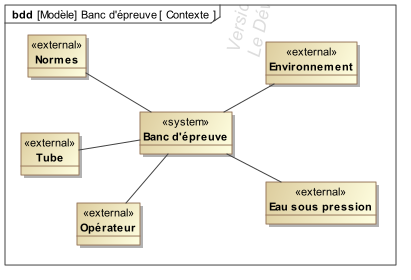
\includegraphics[width=0.7\linewidth]{img/Banc_Contexte}
\end{center}

\begin{center}
	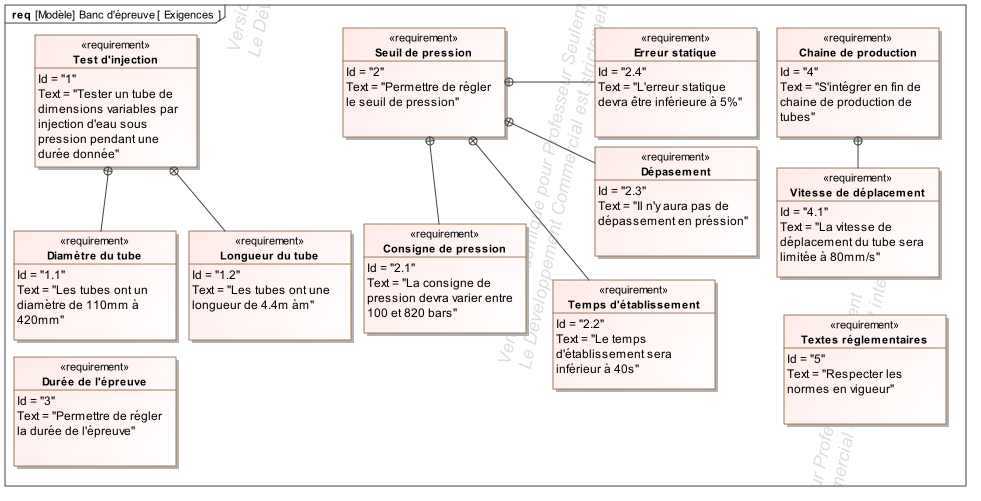
\includegraphics[width=0.9\linewidth]{img/Banc_Exigences}
\end{center}

\subsection{Fonctionnement}

Le banc d'épreuve comporte 4 zones.

\begin{center}
	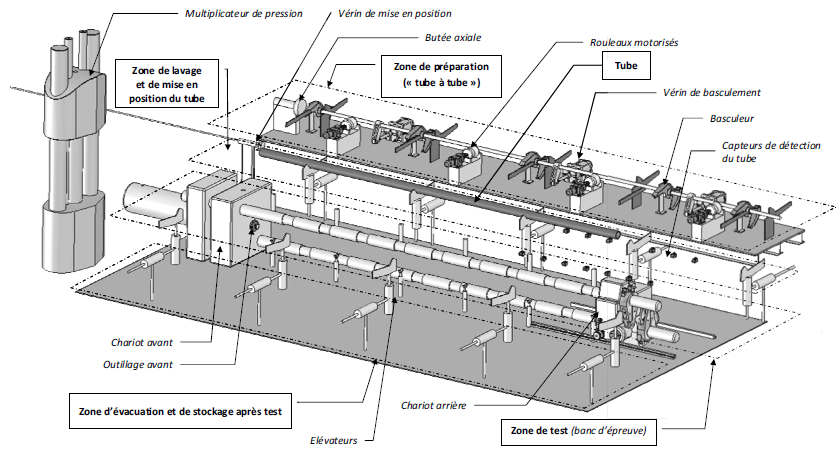
\includegraphics[width=0.9\linewidth]{img/Annexe1}
\end{center}

\subsubsection{Zone de préparation du tube à tester}

Les tubes sont stockés sur des \textbf{rampes de stockage} en légère pente, c'est la gravité qui les fait rouler les uns derrière les autres. Lorsqu'un tube est emmené en zone de préparation, le suivant se met  naturellement à sa place en attente.

\begin{center}
	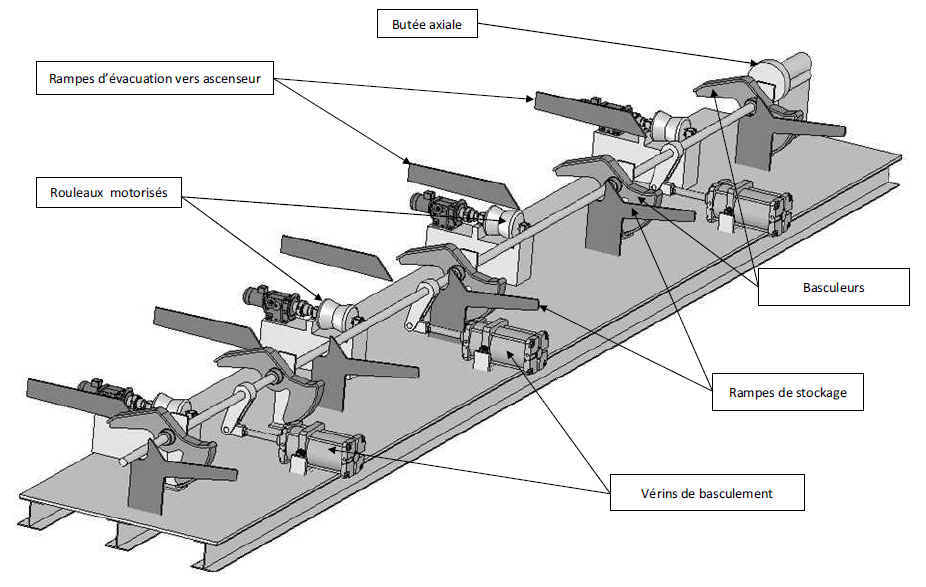
\includegraphics[width=0.9\linewidth]{img/Annexe2}
\end{center}


La préparation consiste à positionner correctement le tube sur le banc et se fait en trois temps:
\begin{itemize}
 \item un système dit \og tube-à-tube \fg composé de cinq \textbf{basculeurs} déstocke un tube pour le placer sur un train de \textbf{rouleaux motorisés},
 \item les rouleaux entrainent le tube axialement jusqu'à ce que son extrémité avant soit placée contre la \textbf{butée axiale},
 \item puis le même système \og tube-à-tube \fg place le tube sur les \textbf{rampes d'évacuation} vers un ascenseur.
\end{itemize}

Cet ascenseur descend ensuite le tube sur un poste de lavage et de mise en position.

\subsubsection{Zone de lavage et de mise en position du tube à tester}

Le lavage se fait sous des jets contrôlés par une soupape à commande pneumatique, à une pression de 14 bars.

La mise en position consiste à faire glisser le tube vers l'arrière à l'aide d'un vérin hydraulique. Sept capteurs de proximité sont disposés sur ce poste le long du tube. Le vérin cesse de déplacer le tube lorsqu'un capteur change d'état en détectant l'extrémité arrière du tube. La mise en position permet de
déterminer la longueur du tube à tester et de définir sa position pendant le test.

\subsubsection{Zone de test du tube à tester (mise sous pression)}

Le tube est ensuite placé dans l'axe du banc d'épreuve grâce aux \textbf{élévateurs}. Le banc d'épreuve est essentiellement constitué d'un chariot avant et d'un chariot arrière, chacun est muni de l'outillage adapté au diamètre des tubes. Avant la mise en place du tube sur le banc, le chariot arrière est mis en position à partir de l'information \og position du tube \fg obtenue lors de la mise en position. Le déplacement du chariot arrière est généré à partir d'un moteur hydraulique, d'un réducteur de vitesse à engrenages et toue et vis sans fin et d'une crémaillère. Le chariot est verrouillé dans cette position par des pinces.

Le tube est alors placé sur le banc. Le chariot avant se déplace ensuite en plaquant le tube sur le chariot arrière, les outillages s'adaptent aux extrémités du tube pour le fermer. Le déplacement du chariot avant est obtenu par vérins hydrauliques.

Le tube est alors rempli d'eau en basse pression amenée au travers du chariot avant. Pendant cette période de remplissage, la purge d'air du tube est assurée par deux soupapes à commandes hydrauliques. L'eau haute pression est fournie par un \textbf{multiplicateur} de pression. Durant l'épreuve, le tube est maintenu en position par un système de clamage et l'outillage avant maintient une pression axiale sur le tube pour garantir l'étanchéité aux extrémités.

A la fin du temps de l'épreuve, la décompression de l'eau est assurée par un clapet de décompression à commande hydraulique monté sur une traverse, le tube est vidé et libéré par le recul des deux chariots.

\subsubsection{Zone d'évacuation et de stockage après test}

Le tube vidé est alors évacué vers un ascenseur de sortie qui sera également poste d'égouttage.

\subsection{Étude de la fonction \og Préparer le tube \fg}

Le système \og tube à tube \fg défini en annexes 2 et 3 remplit deux fonctions :
\begin{itemize}
 \item déstocker le tube pour le placer sur une ligne de rouleaux motorisés qui va translater le tube axialement jusqu'à la butée pour le mettre en position de référence afin de permettre la suite des opérations,
 \item transférer le tube sur une rampe d'évacuation vers un ascenseur.
 
Le système est constitué de trois vérins pneumatiques qui, par l'intermédiaire de leviers, provoquent la rotation d'un arbre relié aux 5 basculeurs qui vont déplacer le tube.
\end{itemize}

Lors des différentes phases de travail du \og tube à tube \fg, il se produit un transfert du poids du tube sur le basculeur et les différents éléments de soutien du tube.

Les schémas de la Figure 4 représentent les quatre phases de ce transfert de charge.
\begin{itemize}
 \item Position I : début de la prise en charge du tube par le basculeur sur la rampe de stockage.
 \item Position II : le tube est déposé sur les galets moteurs.
 \item Position III : début d'évacuation du tube vers la rampe d'évacuation,
 \item Position IV : fin d'évacuation, le tube va quitter le basculeur pour la rampe d'évacuation.
\end{itemize} 

\begin{center}
	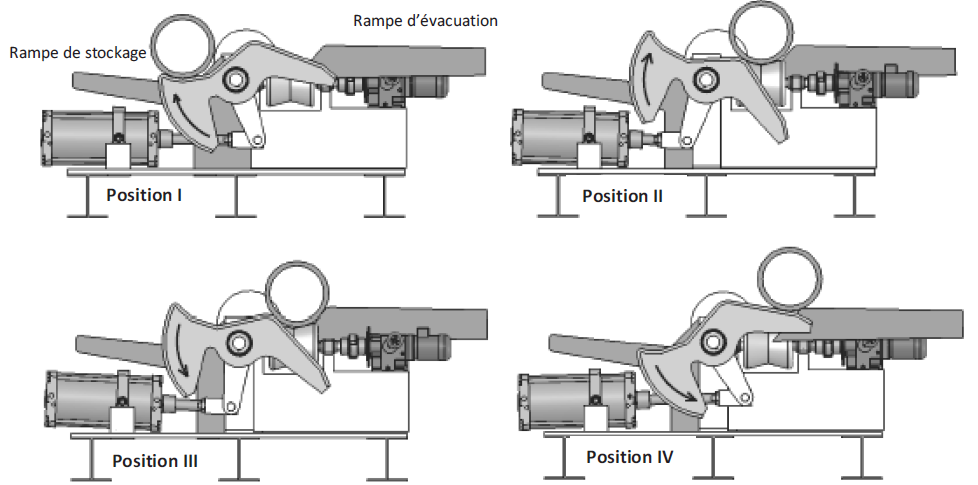
\includegraphics[width=0.9\linewidth]{img/Banc_fig02}
\end{center}

\subsubsection{Modèle d'étude}
Le schéma cinématique proposé pour l'étude est donné par la figure suivante. On y retrouve :
\begin{itemize}
 \item le bâti 0,
 \item le corps de vérin 3,
 \item la tige de vérin 2,
 \item le basculeur 1 composé du levier de commande, de l'arbre et du basculeur.
\end{itemize}

\begin{minipage}{0.6\linewidth}
	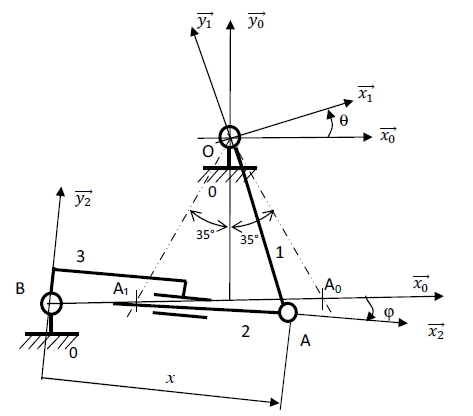
\includegraphics[width=0.9\linewidth]{img/Annexe3}
\end{minipage}
\hfill
\begin{minipage}{0.35\linewidth}
$\overrightarrow{OA}=-R.\overrightarrow{y_1}$, avec $R=400mm$, $\overrightarrow{BA}=x.\overrightarrow{x_2}$

$\overrightarrow{OB}=-h.\overrightarrow{y_0}-d.\overrightarrow{x_0}$.
\end{minipage}

Un repère $R_i$ est attaché à chacun des solides $S_i$.

La position du basculeur $1$ par rapport au bâti $0$ est définie par l'angle $\theta=(\overrightarrow{x_0},\overrightarrow{x_1)}$.

La position de la tige de vérin 2 par rapport au bâti 0 est définie par l'angle $\phi=(\overrightarrow{x_0},\overrightarrow{x_2)}$.

Durant la phase de déstockage, la position $\theta$ du basculeur varie de $+35\degres$ à $-35\degres$.

Le vérin part d'une position horizontale (le point $A$ est en $A_0$), pour arriver de nouveau à l'horizontal en fin de déstockage (le point $A$ est alors en $A_1$).

\subsubsection{Détermination de la course du vérin}

\paragraph{Question 1:} Calculer $h$ pour obtenir les amplitudes de mouvement souhaitées. Calculer alors la course $c$ du vérin.

\paragraph{Question 2:} Déterminer la vitesse de rotation $\dot{\theta}$ en fonction de $\dot{x}$.

\newpage

\section{Chaudière à bois déchiqueté (AADN PTSI 2010)}

\subsection{Présentation générale}

Dans le cadre du \og Grenelle de l'environnement \fg et de la mise en place de la \og taxe carbone \fg, l'avenir du chauffage est conditionné au fait que la biomasse est neutre en dégagement de $CO_2$.

HARGASSNER développe la technologie du chauffage au bois déchiqueté et aux granulés de bois dans le but de concilier un chauffage à la fois écologique et confortable d'utilisation.

L'entreprise est devenue un leader en matière de technique innovante, de développement, de service, de qualité et de longévité dans le domaine du chauffage au bois.

L'étude porte sur la chaudière $HSV 3$, alimentée en bois déchiqueté, qui développe une puissance de chauffe de $25$ à $35 kW$.

Le bois déchiqueté est amené jusqu'à la chaudière dans un premier temps à l'aide d'un extracteur à lames puis de la vis d'extraction et enfin par la vis d'introduction. Il est alors brûlé au sein d'un foyer réfractaire développant des gaz dans la chambre de combustion. Les gaz sont dépoussiérés dans la chambre de détente avant de passer dans un échangeur tubulaire équipé de turbulateurs. Ces turbulateurs augmentent l'efficacité de l'échangeur et permettent son nettoyage automatique.

L'échangeur permet le chauffage de l'eau à partir des fumées. Une vis de dépoussiérage et une vis de décendrage, associées aux turbulateurs évacuent automatiquement les cendres et les suies dans un cendrier.

\subsection{Présentation du système}

\begin{center}
	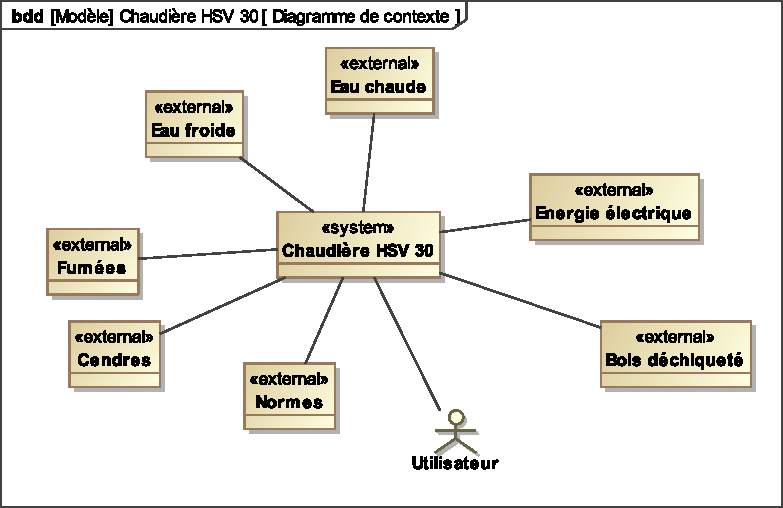
\includegraphics[width=0.8\linewidth]{img/Chaudiere_Contexte}

	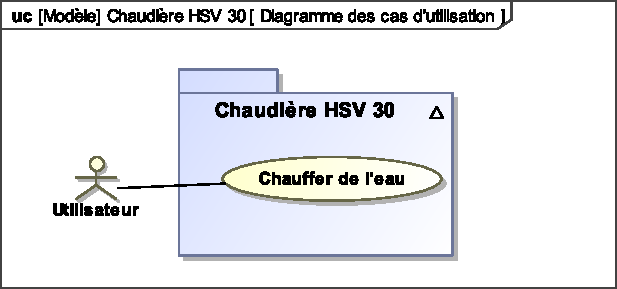
\includegraphics[width=0.6\linewidth]{img/Chaudiere_Cas_utilisation}
\end{center}

\subsection{Vérification de la fonction \og Dépoussiérer, décendrer \fg}

\subsubsection{Mise en situation}

Le système de décendrage nettoie la chaudière à intervalle de temps régulier. La chambre de détente permet la séparation entre les cendres volatiles et les fumées. Les cendres volatiles de dépoussiérage des fumées sont automatiquement transportées et évacuées avec les cendres de combustion grâce d'abord à la vis de dépoussiérage puis à la vis de décendrage, vers le cendrier.

Le nettoyage de l'échangeur à partir des turbulateurs fait tomber les suies sur la vis de dépoussiérage. Celle-ci évacue les suies et les poussières de fumées au dessus de la vis de décendrage. La vis de décendrage évacue les suies, les poussières et les cendres du foyer dans le cendrier. Toutes ces opérations sont réalisées à partir d'un seul motoréducteur (MD).

\paragraph{Etude des mouvements}

Le but de cette partie est d'étudier la relation entre la vitesse de rotation du moteur de décendrage (MD) et la vitesse de translation des turbulateurs. En effet cette vitesse est un élément déterminant pour un nettoyage optimum de l'échangeur qui contribue au bon rendement de la chaudière.

Le cahier des charges stipule que la vitesse maximum des turbulateurs par rapport à l'échangeur soit comprise entre $0,15m.s^{-1}$ et $0,25m.s^{-1}$.

\subsubsection{Étude de la relation entre la rotation du moteur et le mouvement de la tringle de commande 4}

On considère le mécanisme plan (dans le plan ($\overrightarrow{x_0},\overrightarrow{y_0}$)), dans la situation proposée sur le schéma cinématique, et dans le repère $R_0(O,\overrightarrow{x_0},\overrightarrow{y_0},\overrightarrow{z}$).

\begin{center}
	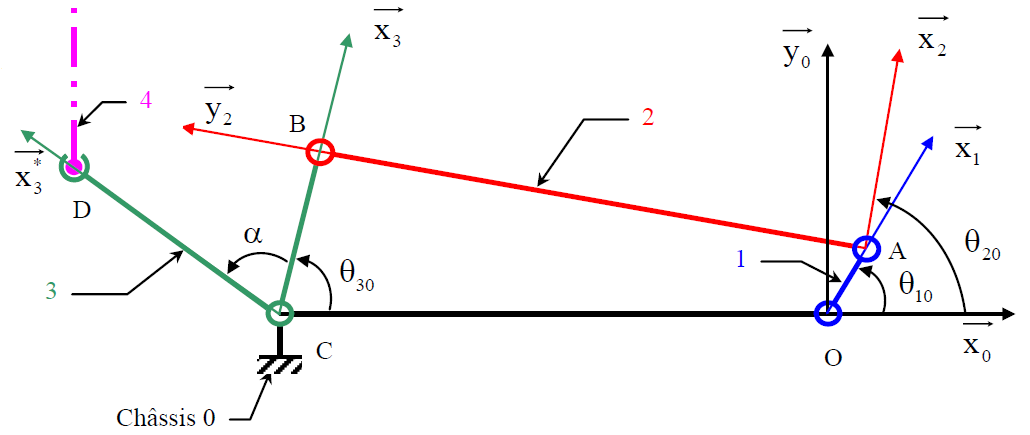
\includegraphics[width=0.6\linewidth]{img/Chaudiere_cinematique}
\end{center}

\begin{itemize}
 \item La manivelle d'entrainement 1 est mise en rotation par le motoréducteur de décendrage (MD), lié au bâti 0, à partir d'une liaison pivot d'axe ($O,\overrightarrow{z}$) à la vitesse de rotation $\omega_{10}$, tel que l'angle $\theta_{10} =(\overrightarrow{x_0},\overrightarrow{x_1})$ et $\overrightarrow{OA} = r.\overrightarrow{x_1}$
 \item Le repère $R_1(O,\overrightarrow{x_1},\overrightarrow{y_1},\overrightarrow{z}$) est lié à la manivelle d'entrainement 1.
 \item La bielle 2 est liée à la manivelle d'entrainement 1 par une liaison pivot d'axe ($A,\overrightarrow{z}$).
 \item Le repère $R_2(A,\overrightarrow{x_2},\overrightarrow{y_2},\overrightarrow{z}$) est lié à la bielle 2. On note l'angle $\theta_{20} =(\overrightarrow{x_0},\overrightarrow{x_2})$.
 \item L'accouplement 3 est lié à la bielle 2 par une liaison pivot d'axe ($B,\overrightarrow{z}$).
 \item Le repère $R_3(B,\overrightarrow{x_3},\overrightarrow{y_3},\overrightarrow{z}$) est lié à l'accouplement 3. On note $\overrightarrow{AB} = l.\overrightarrow{y_2}$.
 \item L'accouplement 3 est lié au bâti 0 par une liaison pivot d'axe ($C,\overrightarrow{z}$).
 \item On note l'angle $\theta_{30} =(\overrightarrow{x_0},\overrightarrow{x_3})$ et $\overrightarrow{BC} = -R.\overrightarrow{x_3}$.
 \item On note $\overrightarrow{CO} = L.\overrightarrow{x_0}$.
\end{itemize}

\paragraph{Question 1:} Écrire la fermeture géométrique pour les centres de liaison O, A, B et C.
En déduire une relation entre $\theta_{30}$ et $\theta_{10}$ uniquement en fonction de r, R, L et l. Cette relation permettrait d'obtenir $\theta_{30}$ en fonction de $\theta_{10}$.

\paragraph{Question 2:} Quelle méthode faudrait-il appliquer pour en déduire la relation entre la vitesse de rotation $\omega_{10}$ de la manivelle 1 par rapport au bâti 0, et la vitesse de rotation $\omega_{30}$ de l'accouplement 3 par rapport au bâti 0 (il n'est pas demandé de calcul).

L'accouplement 3 est formé de deux bras décalés l'un de l'autre d'un angle $\alpha=(\overrightarrow{x_3},\overrightarrow{x^*_3})$
3. La tringle de commande 4 est en liaison pivot d'axe $(D,\overrightarrow{z})$ avec l'accouplement 3 au point D et tel que $\overrightarrow{CD}=d.\overrightarrow{x^*_3}$.

\paragraph{Question 3:} Déterminer la vitesse du point D appartenant à l'accouplement 3 dans son mouvement par rapport au bâti 0 notée $\overrightarrow{V_{D\in 3/0}}=V_{D30}.\overrightarrow{y^*_3}$ en fonction de la vitesse de rotation $\omega_{30}$ et en projection dans le repère $R_0(O,\overrightarrow{x_0},\overrightarrow{y_0},\overrightarrow{z})$.

Pour la suite, dans l'étude du mouvement simplifié, on ne tiendra pas compte de la composante sur $\overrightarrow{x_0}$.

\subsection{Étude du mouvement entre la tringle de commande 4 et les turbulateurs 8 et 9}

On considère le mécanisme plan (dans le plan $(\overrightarrow{y_0},\overrightarrow{z})$), dans la situation telle que modélisée schématiquement sur le schéma cinématique, dans le repère $R_0(O,\overrightarrow{x_0},\overrightarrow{y_0},\overrightarrow{z})$.

\begin{center}
	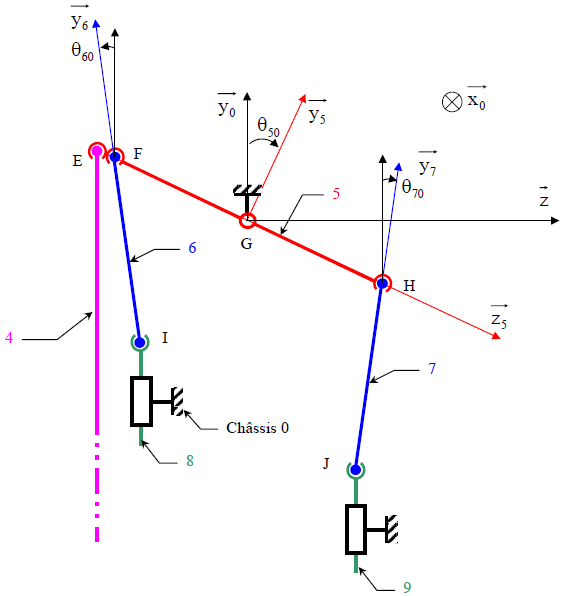
\includegraphics[width=0.7\linewidth]{img/Chaudiere_cinematique_2}
\end{center}

L'axe de commande 5 est mis en rotation par la tringle de commande 4, telle que la vitesse du point E lié à l'axe de commande 5 par rapport au bâti 0 est : $\overrightarrow{V_{E\in 5/0}}=V_{E50}.\overrightarrow{y_5}$.

L'axe de commande 5 est en liaison pivot avec le bâti 0 d'axe $(G,\overrightarrow{x_0})$.

Les plaques support 6 et 7, sont en liaison sphérique avec l'axe de commande 5 respectivement de centre F et H.

Les turbulateurs 8 et 9 sont en liaison sphérique avec les plaques support 6 et 7 respectivement de centre I et J, et en liaison glissière avec l'échangeur lié au bâti 0 de direction respective $\overrightarrow{y_0}$ et $\overrightarrow{y_0}$.

A partir d'une étude cinématique graphique et dans la position définie sur le document réponse, donner les rapports qui existent entre $\overrightarrow{V_{E\in 5/0}}=V_{E50}.\overrightarrow{y_5}$ et :

\paragraph{Question 4:}  D'une part la vitesse du point I appartenant au turbulateur 8 dans son mouvement par rapport au bâti 0 $\overrightarrow{V_{I\in 8/0}}=V_{I80}.\overrightarrow{y_0}$;

\paragraph{Question 5:} d'autre part la vitesse du point J appartenant au turbulateur 9 dans son mouvement par rapport au bâti 0 $\overrightarrow{V_{J\in 9/0}}=V_{J90}.\overrightarrow{y_0}$.

Justifier les constructions.

\subsubsection{Étude du mouvement simplifié de la tringle de commande 4}

Nota : les deux schémas proposés dans cette partie définissent la géométrie du système pour un même instant, lorsque les turbulateurs se déplacent aux vitesses maximum (déterminé au cours d'une autre étude).

\begin{center}
	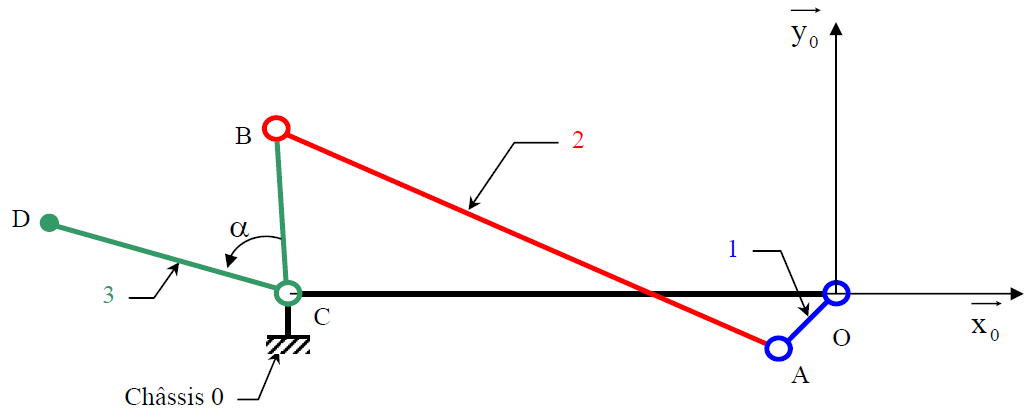
\includegraphics[width=0.7\linewidth]{img/Chaudiere_cinematique_3}
\end{center}

Les dimensions des mécanismes sont telles que :
\begin{itemize}
 \item DE = 1 150 mm sur la tringle de commande 4,
 \item CD = d = 120 mm sur l'accouplement 3,
 \item EG = 92 mm sur l'axe de commande 5.
\end{itemize}

\begin{center}
	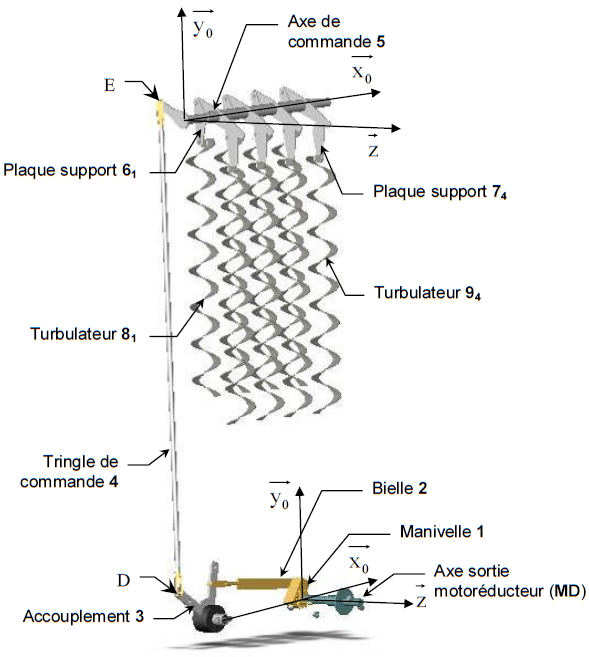
\includegraphics[width=0.6\linewidth]{img/Chaudiere_cinematique_4}
\end{center}

\paragraph{Question 6:} A partir du schéma fourni à l'échelle 1/3 sur le document réponse, tracer les deux positions extrêmes du point D appartenant à l'accouplement 3 dans son mouvement par rapport au bâti 0 : D0 et D1. Préciser la méthode.

\paragraph{Question 7:} En comparant la longueur de la tringle de commande 4 par rapport aux autres dimensions, quelle approximation peut-on faire quant au mouvement de la tringle de commande 4 par rapport au bâti 0.

\paragraph{Question 8:} A partir des positions extrêmes obtenues dans la question précédente, du schéma fourni à l'échelle 1/2 sur le document réponse et de l'approximation précédente, tracer les deux positions extrêmes approximatives du point E appartenant à l'axe de commande 5 dans son mouvement par rapport au bâti 0 : respectivement $E_0$ et $E_1$.

\subsubsection{Étude de la relation entre la rotation du moteur et la translation des turbulateurs 8 et 9}

Dans la position du système donnée pour l'étude de cinématique graphique et les épures, la relation entre $\omega_{30}$ et $\omega_{10}$ est telle que $\omega_{30}=K_1.\omega_{10}$ avec $\omega_{10}=4rad.s^{-1}$, $\theta_{30}=95\degres$, et $\alpha=70\degres$.

Dans les applications numériques, pour un angle compris entre $160\degres$ et $180\degres$, on prendra son cosinus équivalent à $-1$.

\paragraph{Question 9:} En déduire de manière littérale la composante sur $\overrightarrow{y_0}$ de la vitesse de la tringle de commande 4 par rapport au bâti 0 : $V_{40}$ en fonction de $K_1$, $\omega_{10}$, et $d$.

\paragraph{Question 10:} Vérifier que les valeurs absolues approchées des vitesses maximum de translation des turbulateurs 8 et 9 sont conformes au cahier des charges. Pour cela $K_1=-\dfrac{1}{2}$, cette valeur ayant été obtenue à partir d'une étude annexe.

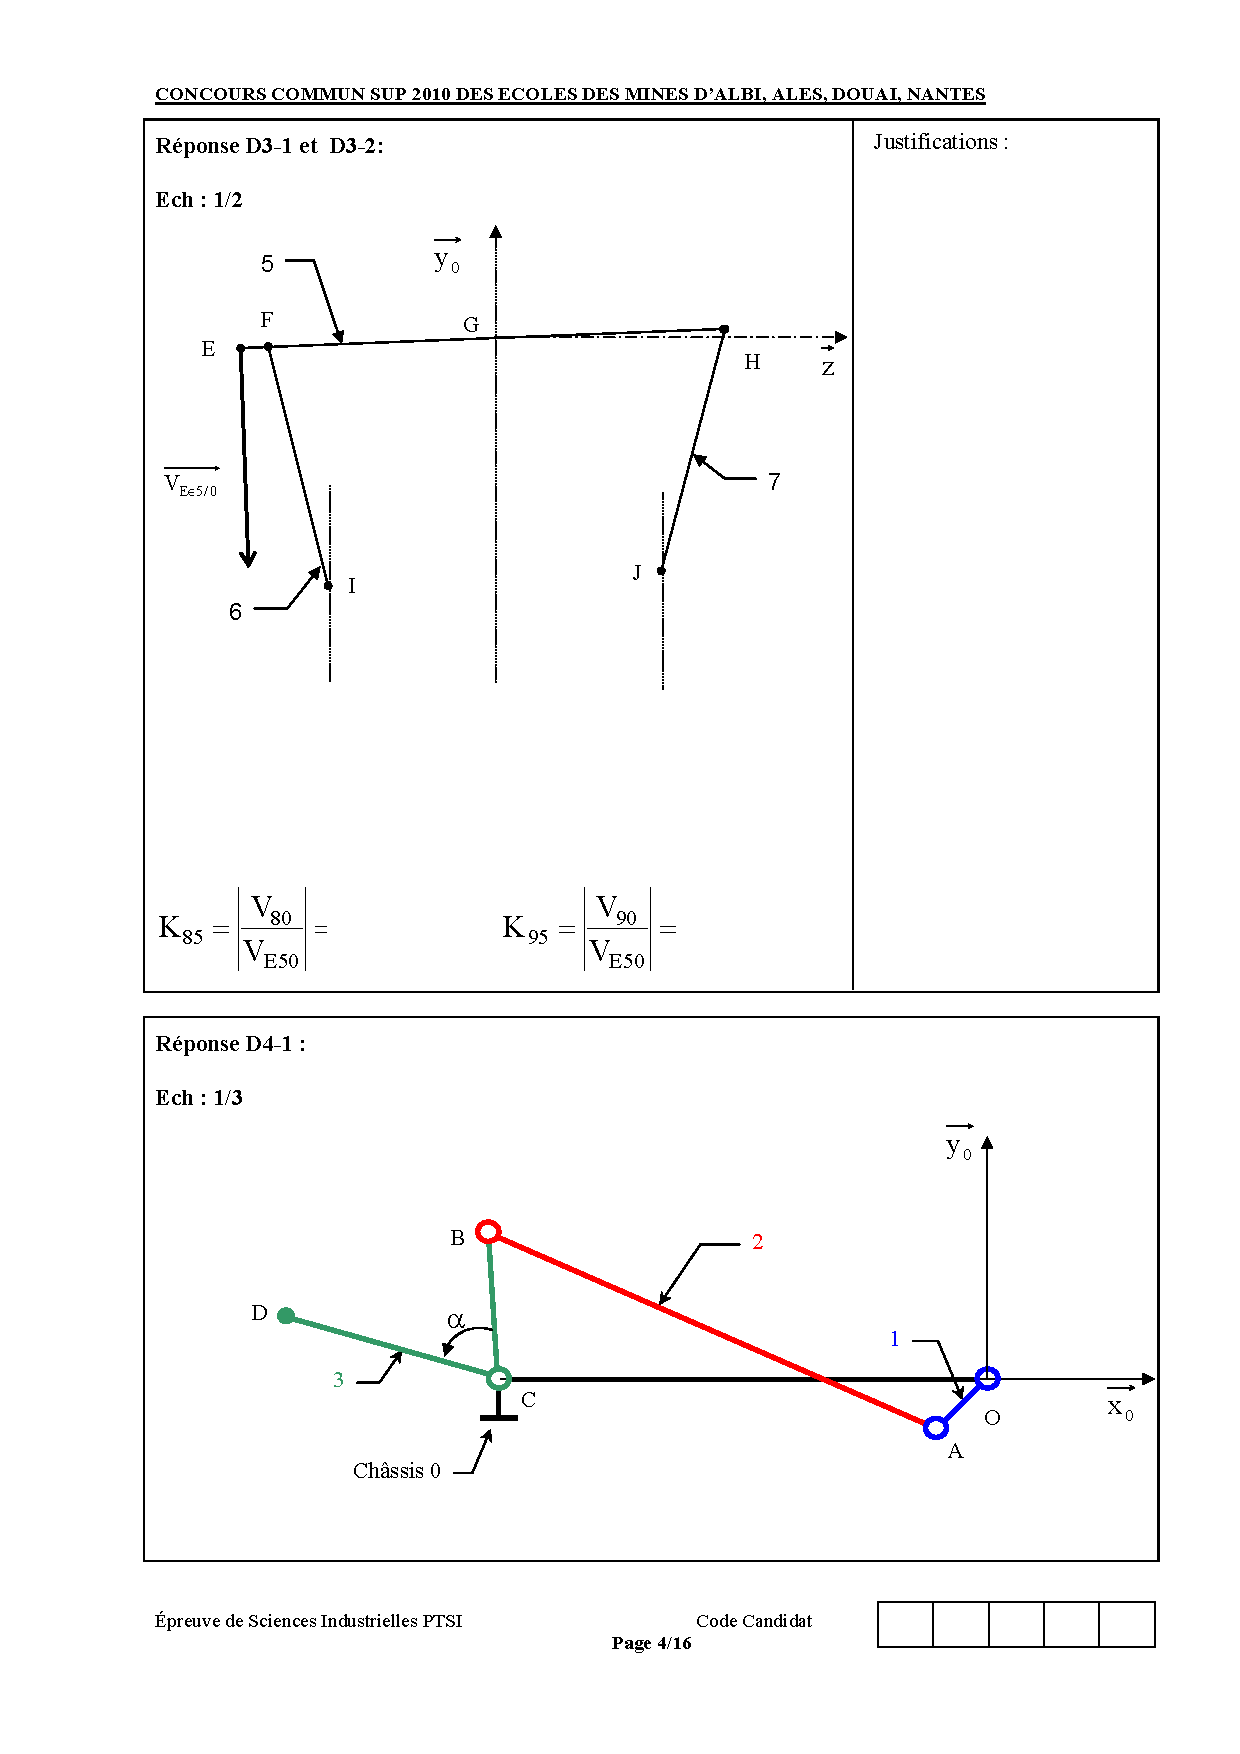
\includepdf{img/Doc_rep_06-TD02.pdf}

\section{Mécanisme de commande de pompe doseuse}

Un mécanisme de pompe doseuse est entraîné par un moto-réducteur (non représenté sur le dessin d'ensemble) auquel est accouplé l'excentrique 41. La course du piston 66 est modifiée lorsqu'on tourne le volant 8.

On étudie la partie commande de la pompe. Pour une étude cinématique, le mécanisme peut être ramené à un problème plan (de normale $\overrightarrow{z_0}$) schématisé sur la figure \ref{commande_figure_1}.

\begin{figure}[!ht]
\begin{center}
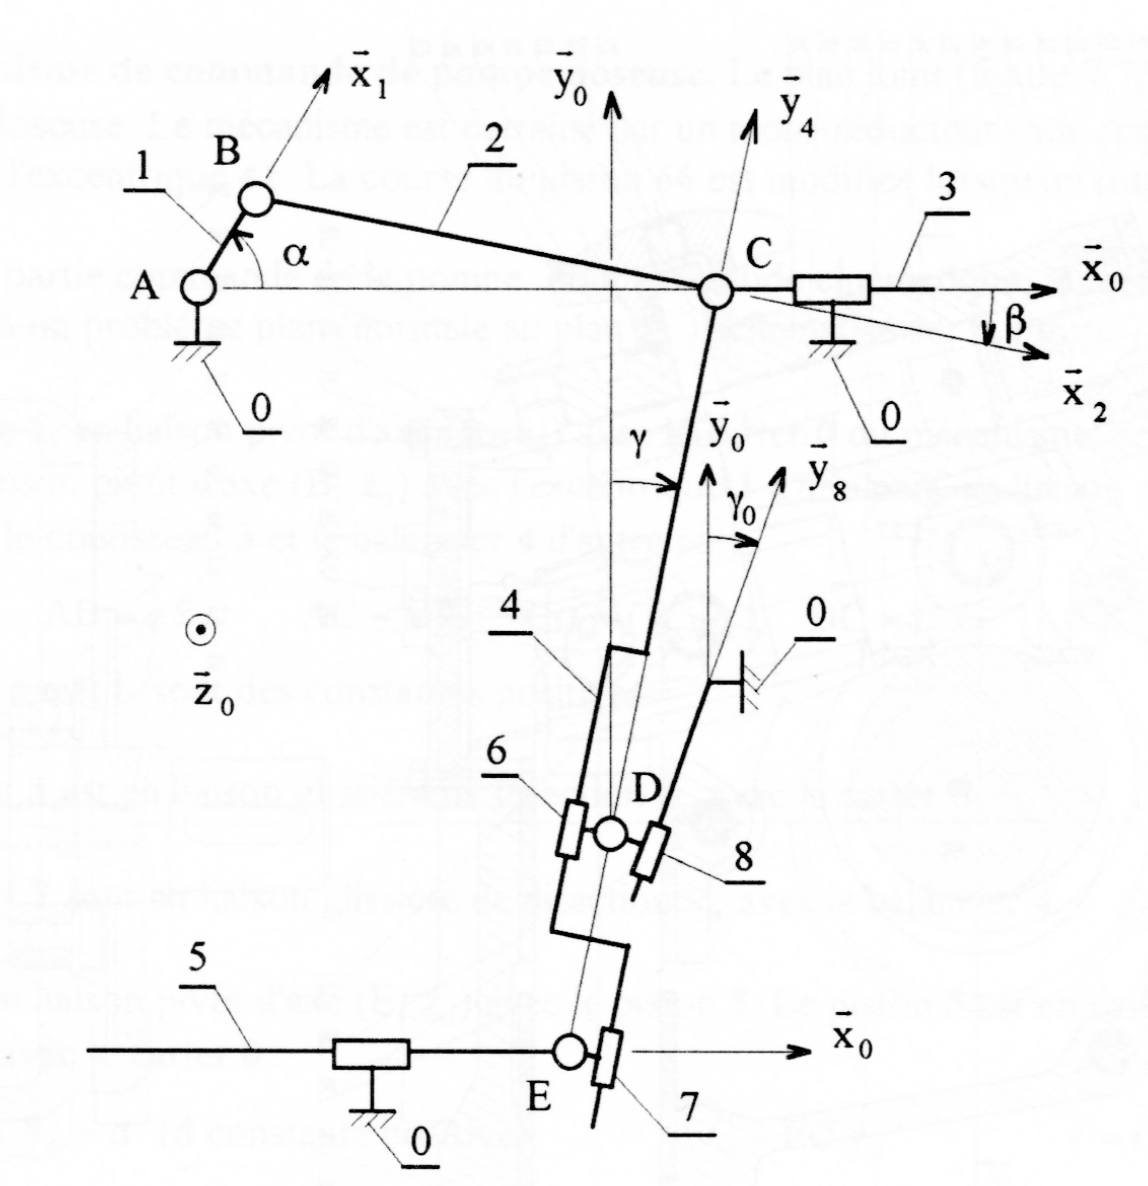
\includegraphics[width=0.6\linewidth]{img/commande_figure_1}
\caption{Schéma cinématique de la commande de la pompe}
\label{commande_figure_1}
\end{center}
\end{figure}

L'excentrique \textbf{1}, en liaison pivot d'axe $(A,\overrightarrow{z_0})$ avec le carter \textbf{0}, commande la bielle \textbf{2}, elle-même en liaison pivot d'axe $(B, \overrightarrow{z_0})$ avec l'excentrique \textbf{1} d'une part, et en liaison pivot d'axe $(C,\overrightarrow{z_0})$ avec le  coulisseau \textbf{3} et le balancier \textbf{4} d'autre part.

Le coulisseau \textbf{3} est en liaison glissière de direction $\overrightarrow{x_0}$ avec le carter \textbf{0}.

Deux dés \textbf{6} et \textbf{7} sont en liaison glissière de direction $\overrightarrow{y_4}$ avec le balancier \textbf{4}.

Le dé \textbf{7} est en liaison pivot d'axe $(E,\overrightarrow{z_0})$ avec le piston \textbf{5}. Le piston \textbf{5} est en liaison glissière de direction $\overrightarrow{x_0}$ avec le carter \textbf{0}.

Le dé \textbf{6} est en liaison pivot d'axe $(D,\overrightarrow{z_0})$ avec le coulisseau \textbf{8}. Les points C, D et E sont alignés.

Le coulisseau \textbf{8} est en liaison glissière de direction $\overrightarrow{y_8}$ avec le carter \textbf{0}.

Lorsqu'on fait varier (en fonctionnement) la position du coulisseau \textbf{8} par rapport au carter \textbf{0}, la position de l'axe $(D,\overrightarrow{z_0})$ par rapport au carter \textbf{0} est changée, et la course du piston \textbf{5} est modifiée.

Pour que le point mort avant (ou gauche) du piston \textbf{5} ait toujours la même position quelle que soit la course du piston \textbf{5}, on a, pour $\alpha=0$, $\gamma=\gamma_0$, c'est à dire $\overrightarrow{y_4}$ et $\overrightarrow{y_8}$ parallèles. Dans cette position, on pose $\overrightarrow{ED}=\lambda.\overrightarrow{y_8}$.

\newpage

On pose les données suivantes :

\begin{minipage}{0.3\linewidth}
\begin{itemize}
 \item $\overrightarrow{AB}=e.\overrightarrow{x_1}$,
 \item $\overrightarrow{AC}=x.\overrightarrow{x_0}$,
 \item $\alpha=(\overrightarrow{x_0}, \overrightarrow{x_1})$,
 \item $\overrightarrow{BC}=L.\overrightarrow{x_2}$,
 \item $\beta=(\overrightarrow{x_0}, \overrightarrow{x_2})$,
 \item $\overrightarrow{EA}.\overrightarrow{y_0}=d$,
 \item $\overrightarrow{EC}=EC.\overrightarrow{y_4}$,
\end{itemize}
\end{minipage}\hfill
\begin{minipage}{0.65\linewidth}
\begin{itemize}
 \item $\gamma=(\overrightarrow{y_0}, \overrightarrow{y_4})$,
 \item $\gamma_0=(\overrightarrow{y_0}, \overrightarrow{y_8})$,
 \item $d$, $e$ et $L$ sont des constantes positives,
 \item $\gamma_0$ est une constante (une fois le réglage effectué),
 \item $e=15mm$, $L=70mm$, $d=120mm$, $cos\gamma_0=0,96$ et $30mm\leq\lambda\leq60mm$.
\end{itemize}
Hypothèse : on suppose $\lambda$ constant dans toutes les études qui suivent.
\end{minipage}

\subsection{Première partie : étude des paramètres}

\paragraph{Question 1:} Déterminer la course du coulisseau \textbf{3} et faire l'application numérique.

\paragraph{Question 2:} Déterminer la course $c$ du piston \textbf{5} en fonction de $d$, $e$, $\lambda$ et $\gamma_0$. Faire l'application numérique pour $\lambda=30mm$, $\lambda=45mm$ et $\lambda=60mm$.

\paragraph{Question 3:} Déterminer $x$ et $\beta$ en fonction de $e$, $L$ et $\alpha$.

\paragraph{Question 4:} Déterminer $\gamma$ en fonction de $e$, $L$, $d$, $\lambda$, $\gamma_0$ et $x$.

\subsection{Deuxième partie : Étude graphique, détermination du vecteur vitesse de translation du piston 5 par rapport au carter 0}

\paragraph{Question 5:} Pour $\alpha=\frac{7\pi}{4}$ construire une épure, respectant les proportions, mettant en place les différents points A, B, C, D et E, expliquer les constructions.

\begin{center}
 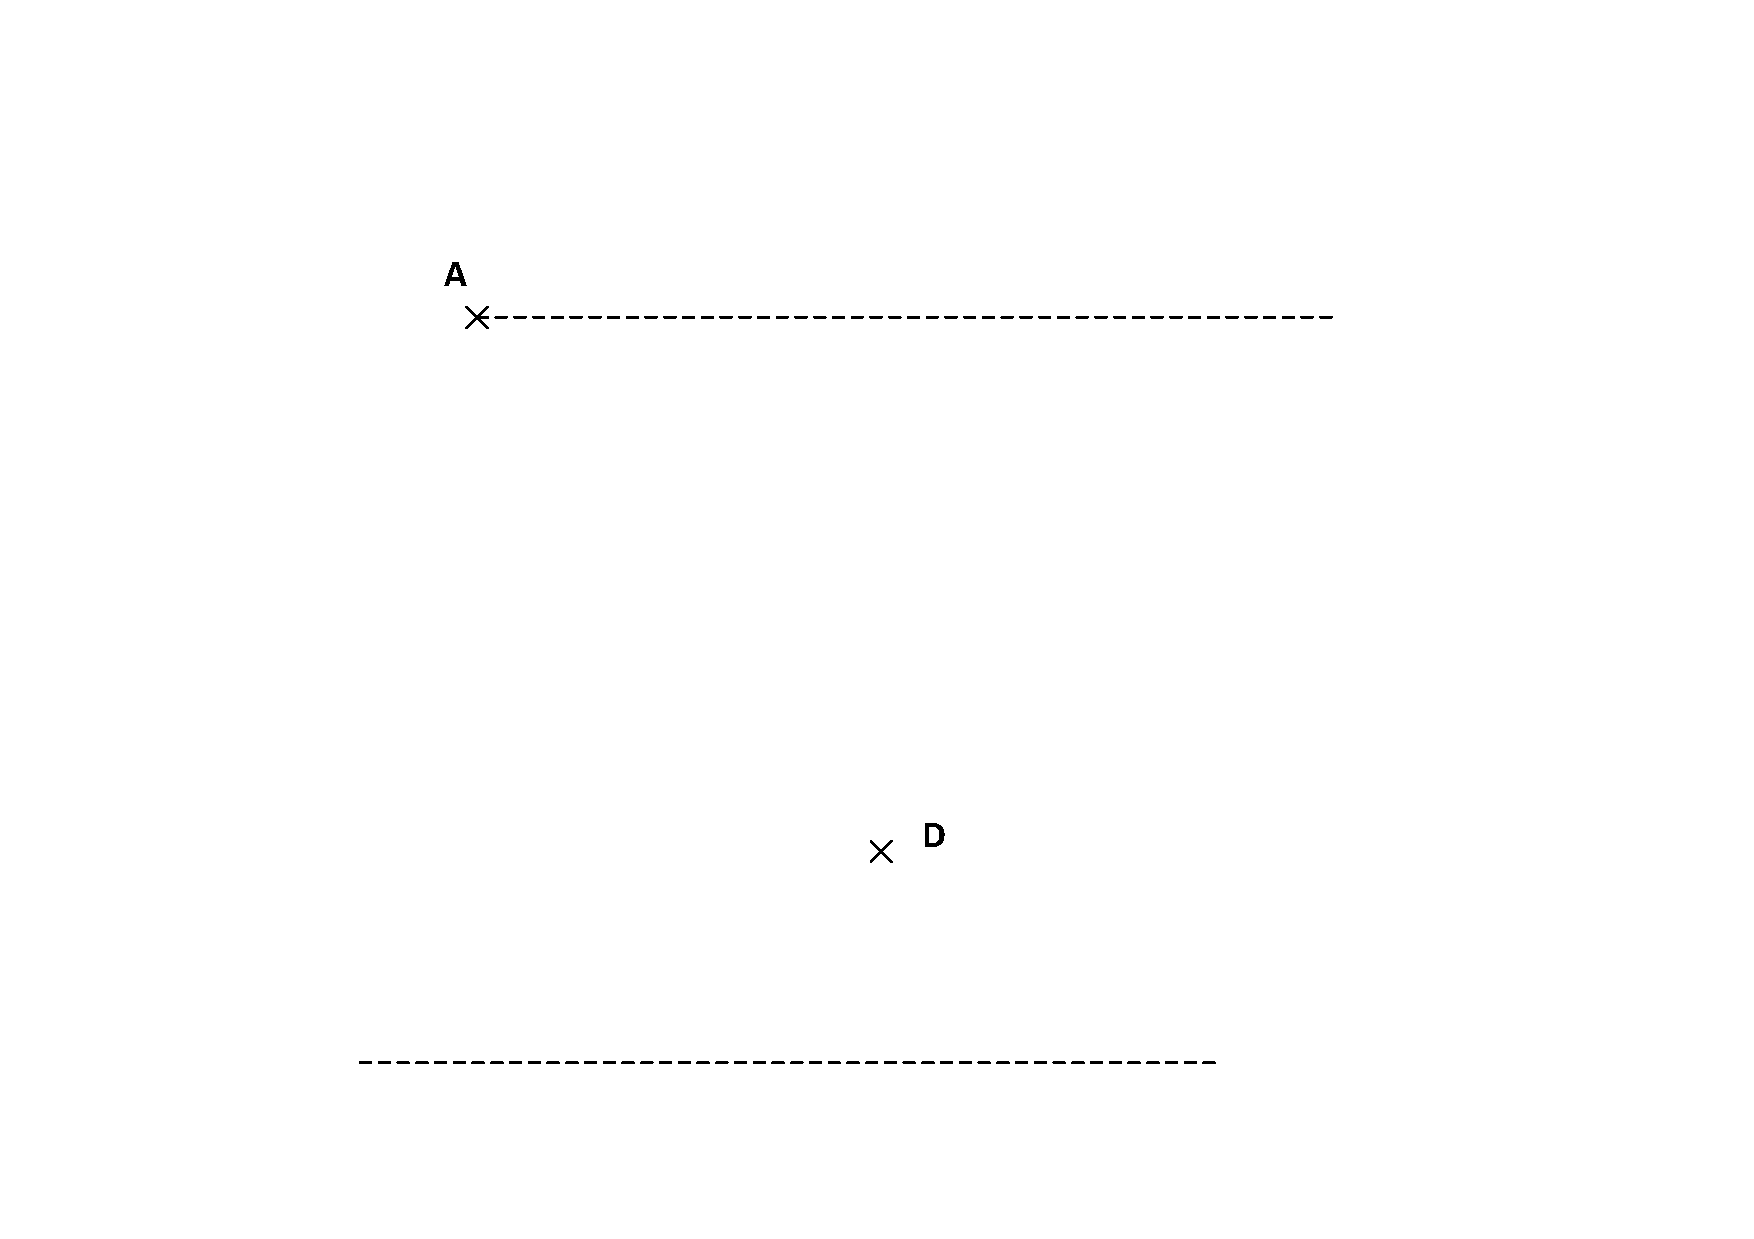
\includegraphics[width=0.8\linewidth]{img/epure}
\end{center}
\paragraph{Question 6:} On suppose que l'excentrique a une fréquence de rotation $N_{10}=90tr/min$. Dans la configuration précédente, déterminer graphiquement $\vec{V}_{E\in 5/0}$. Justifier les constructions.

\subsection{Troisième partie : Étude analytique}

Cette étude a pour but d'aider à l'analyse du comportement du mécanisme, et trouver notamment :
\begin{itemize}
 \item le vecteur vitesse de translation du piston 5 par rapport au bâti 0 pour connaître le débit instantané de la pompe,
 \item le vecteur vitesse de glissement de points particuliers des liaisons pour prévoir leur comportement (usure, création de film d'huile),
 \item le vecteur accélération de centre d'inertie en vue d'une étude dynamique.
\end{itemize}

\paragraph{Question 7:} Déterminer le vecteur vitesse $\vec{V}_{E\in 5/0}$ en fonction de $d$, $\lambda$, $\gamma_0$ et $\dot{x}$.

On pose $\vec{V}_{E\in 5/0}=V_{E\in 5/0}.\overrightarrow{x_0}$.

On donne le graphe de $V_{ E\in 5/0}$ en fonction de $\alpha$ pour $\lambda=30mm$, $\lambda=45mm$ et $\lambda=60mm$. (figure \ref{commande_figure_2}).

\begin{figure}[!ht]
\begin{center}
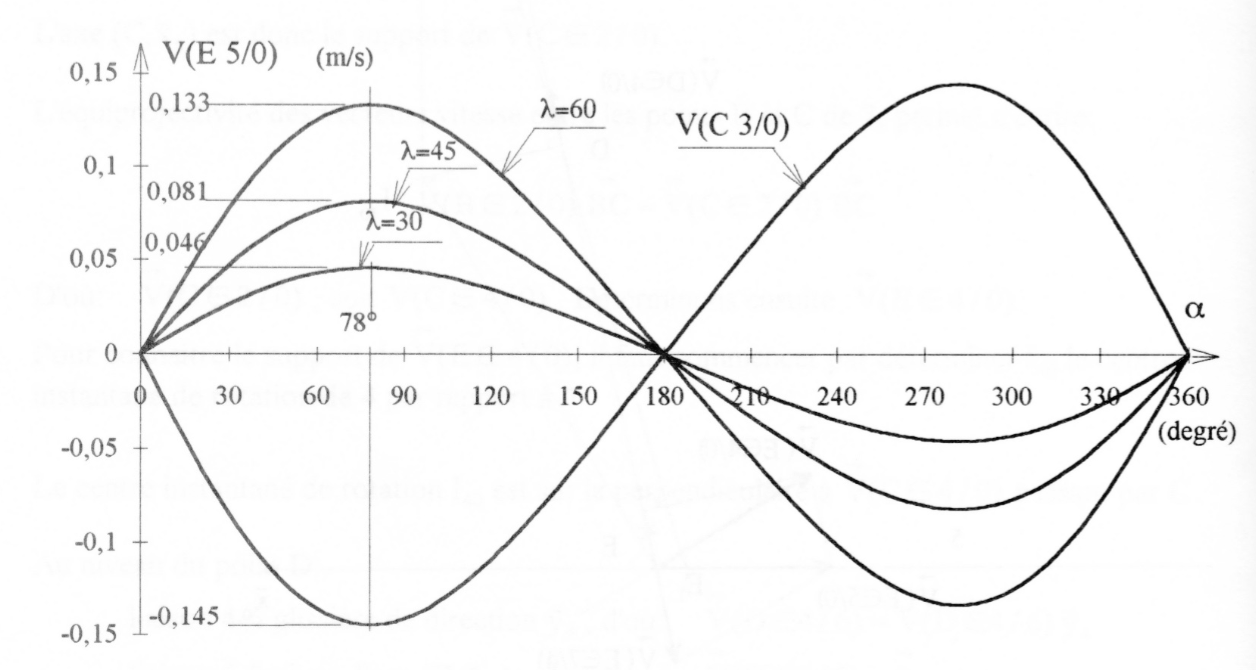
\includegraphics[width=0.6\linewidth]{img/commande_figure_2}
\caption{$V_{ E\in 5/0}$ en fonction de $\alpha$}
\label{commande_figure_2}
\end{center}
\end{figure}

\paragraph{Question 8:} Déterminer le vecteur vitesse $\vec{V}_{D\in 4/6}$ en fonction de $\lambda$ et de $\dot{x}$.
affaires sensibles 7
feroni 0
On pose $\vec{V}_{D\in 4/6}=V_{D\in 4/6}.\overrightarrow{y_4}$.

On donne le graphe de $V_{D\in 4/6}$ en fonction de $\alpha$ pour $\lambda = 30 mm$, $\lambda=45mm$ et $\lambda=60mm$. (figure \ref{commande_figure_3}).

\begin{figure}[!ht]
\begin{center}
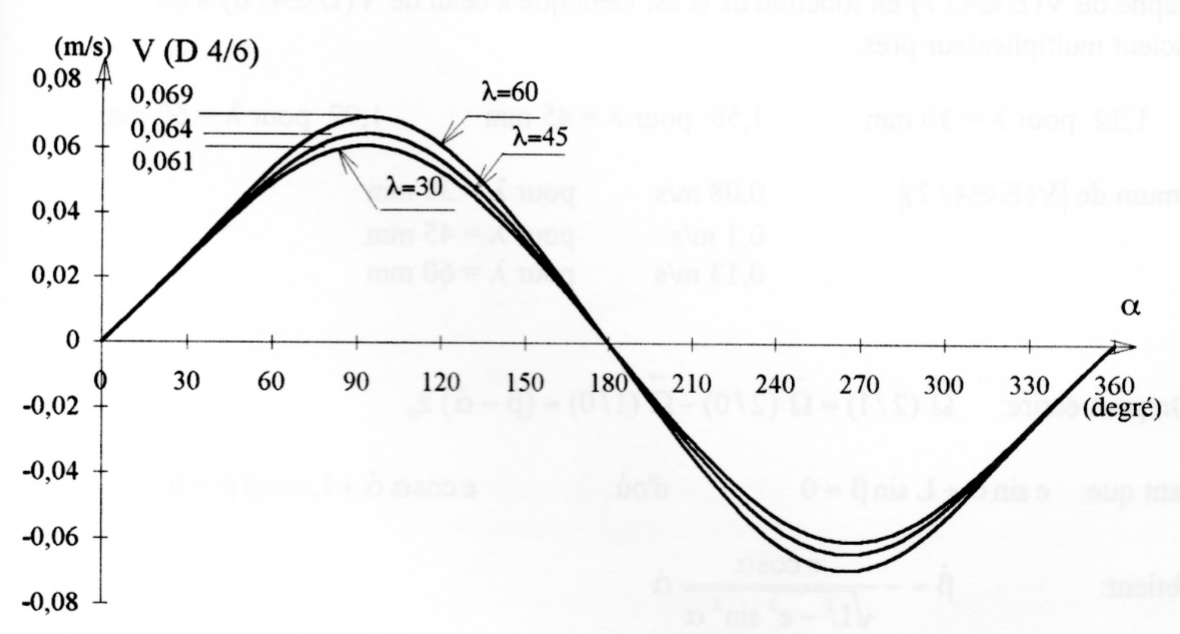
\includegraphics[width=0.6\linewidth]{img/commande_figure_3}
\caption{$V_{D\in 4/6}$ en fonction de $\alpha$}
\label{commande_figure_3}
\end{center}
\end{figure}

\paragraph{Question 9.a:} Déterminer le vecteur vitesse $\vec{V}_{E\in 4/7}$ en fonction de $d$, $\lambda$, $\gamma$, $\gamma_0$ et $\dot{x}$.

On pose $\vec{V}_{E\in 4/7}={V}_{E\in 4/7}.\overrightarrow{y_4}$.
 
\paragraph{Question 9.b:} Indiquer comment déduire du graphe de ${V}_{D\in 4/6}$ en fonction de $\alpha$, le graphe de $\vec{V}_{E\in 4/7}$ en fonction de $\alpha$.

\paragraph{Question 9.c:} Donner la valeur maximum du module de $\vec{V}_{E\in 4/7}$ pour $\lambda=30mm$, $\lambda=45mm$ et $\lambda=60mm$.

\paragraph{Question 10:} Déterminer le vecteur rotation $\overrightarrow{\Omega}_{(2/1)}$ en fonction de $e$, $L$, $\alpha$, $\dot{\alpha}$.

\paragraph{Question 11:} La liaison pivot d'axe $(B, \overrightarrow{z_0})$ entre \textbf{1} et \textbf{2} est réalisée à l'aide d'un excentrique (figure \ref{commande_figure_4}).

\begin{figure}[!ht]
\begin{center}
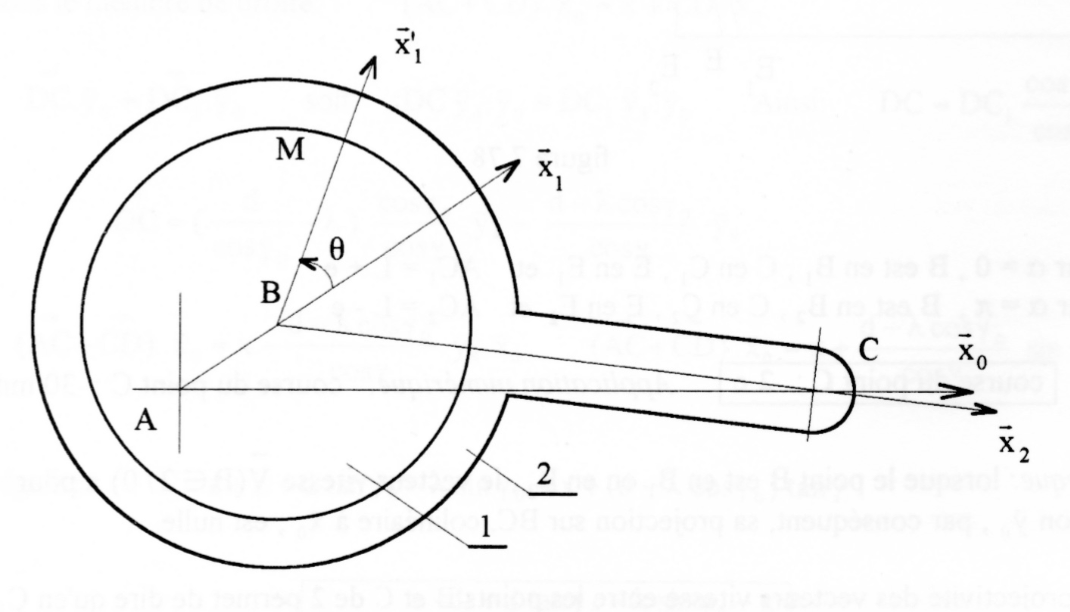
\includegraphics[width=0.6\linewidth]{img/commande_figure_4}
\caption{Liaison pivot d'axe $(B, \vec{z_0})$ entre \textbf{1} et \textbf{2}}
\label{commande_figure_4}
\end{center}
\end{figure}

Déterminer le vecteur vitesse $\vec{V}_{M\in 2/1}$ en fonction de $R$, $\dot{\beta}$ et $\dot{\alpha}$.

\paragraph{Question 12:} Soit $G$ le centre d'inertie du balancier \textbf{4}. On pose $\overrightarrow{GC}=H.\overrightarrow{y_4}$.
Déterminer le vecteur accélération du point $G$ par rapport au carter \textbf{0} $\vec{\Gamma}_{G\in 4/0}$ en fonction de $H$, $\ddot{x}$, $\dot{\gamma}$ et $\ddot{\gamma}$.


\ifdef{\public}{\end{document}}{}

\clearpage

\newpage

\section{Correction}

\subsection{Moteur à explosion}

\paragraph{Question 1:} 

\begin{center}
 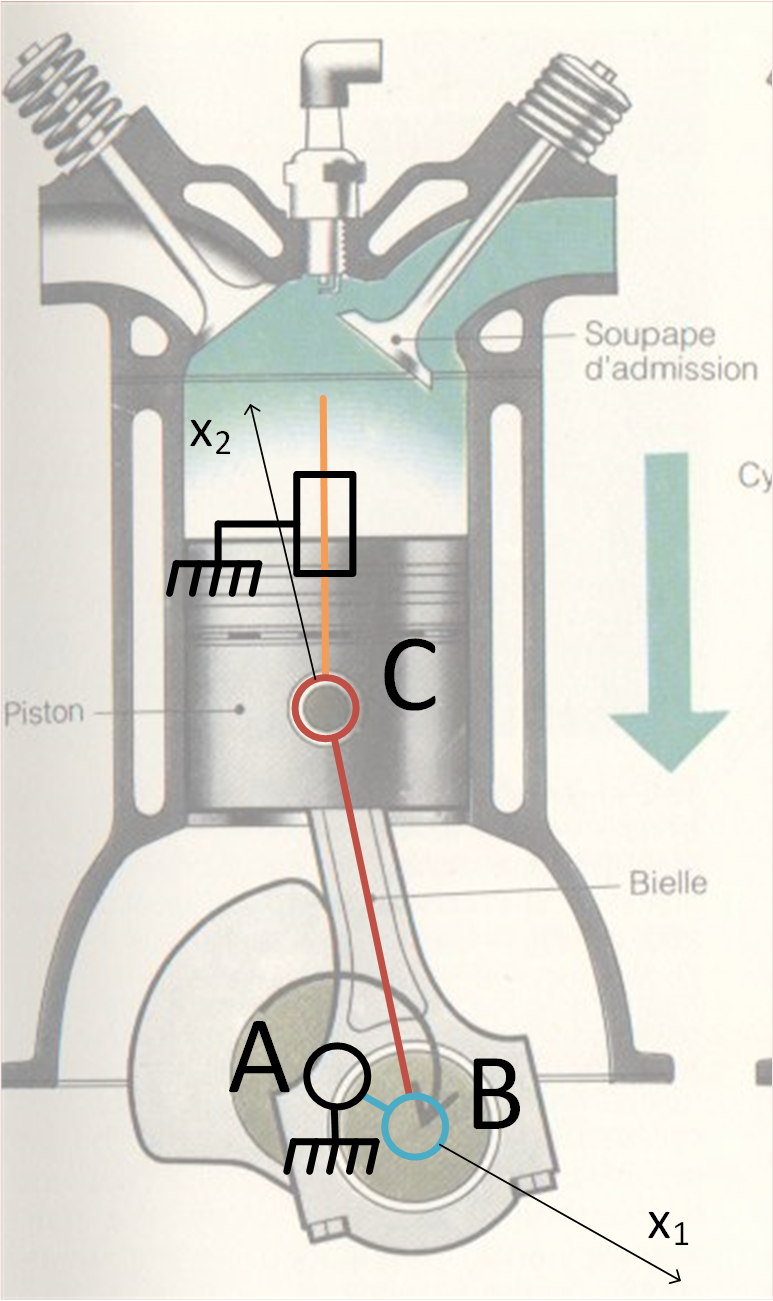
\includegraphics[width=0.3\linewidth]{img/cin_cor}
\end{center}

\paragraph{Question 2:} 

$\overrightarrow{AB}+\overrightarrow{BC}+\overrightarrow{CA}=\overrightarrow{0}$

$l_1.(cos\theta_1.\overrightarrow{x_0}+sin\theta_1.\overrightarrow{y_0})+l_2.(cos\theta_.\overrightarrow{x_0}+sin\theta_2.\overrightarrow{y_0})-l(t).\overrightarrow{y_0}=\overrightarrow{0}$.

Donc, $\left\{\begin{array}{l}
l_1.cos\theta_1+l_2.cos\theta_2=0\\
l_1.sin\theta_1+l_2.sin\theta_2-l(t)=0
\end{array}\right.$

Donc,

$\theta_2=arccos\left(-\frac{l_1}{l_2}.cos\theta_1\right)$

et $l_2^2=(l(t)-l_1.sin\theta_1)^2+(l_1.cos\theta_1)^2$, ainsi, $l(t)=l_1.sin\theta_1+\sqrt{l_2^2-(l_1.cos\theta_1)^2}$

\paragraph{Question 3:} 

$\overrightarrow{V_{B\in1/0}}=l1.\omega_{10}.\overrightarrow{y_1}$
$\overrightarrow{V_{B\in2/0}}=l1.\omega_{10}.\overrightarrow{y_1}$, car $\overrightarrow{V_{B\in2/1}}=\overrightarrow{0}$

$\overrightarrow{V_{C\in2/0}}=\overrightarrow{V_{B\in2/0}}+\overrightarrow{CB}\wedge\overrightarrow{\Omega_{20}}
=l1.\omega_{10}.\overrightarrow{y_1}-l_2.\overrightarrow{x_2}\wedge\omega_{20}.\overrightarrow{z}$

\paragraph{Question 4:}

$\left\{\begin{array}{l}
l_1.\omega_{10}.cos\theta_1+l_2.\omega_{20}.cos\theta_2=0\\
l_1.\omega_{10}.sin\theta_1+l_2.\omega_{20}.sin\theta_2=Vc
\end{array}\right.$

Donc, $Vc=l_1.\omega_{10}.(sin\theta_1-tan\theta_2.cos\theta_1)$

\paragraph{Question 5:} 

$\Gamma_c=l_1*\omega_{10}.\left(\omega_{10}.cos\theta_1-\omega_{20}.\frac{cos\theta_1}{cos\theta_2^2}+\omega_{10}.tan\theta_2.sin\theta_1\right)$

\subsection{Décocheuse industrielle}

\paragraph{Question 1:}

La masse de l'ensemble suit la courbe $p=125-\frac{20}{61}.t$

\begin{center}
 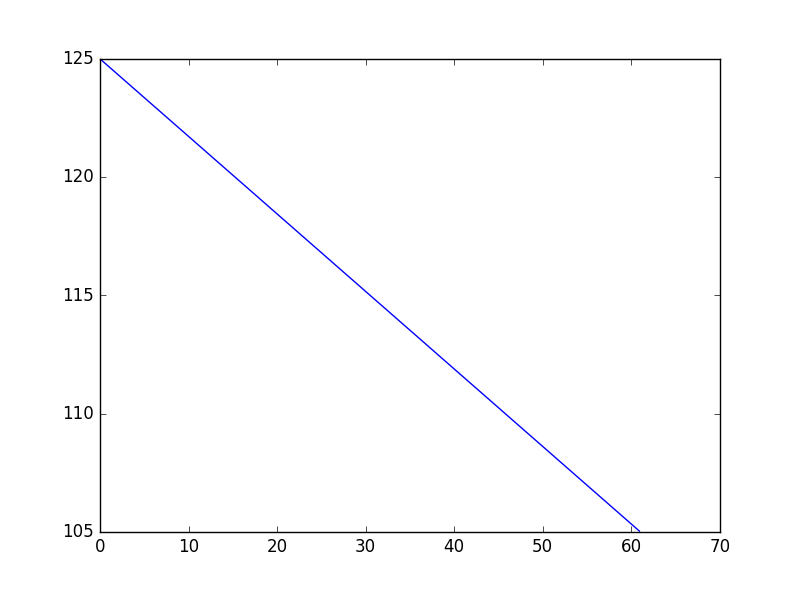
\includegraphics[width=0.3\linewidth]{img/courbe_poids}
\end{center}

\paragraph{Question 2:}

Le mouvement est une translation circulaire.

\paragraph{Question 3:}

\begin{center}
 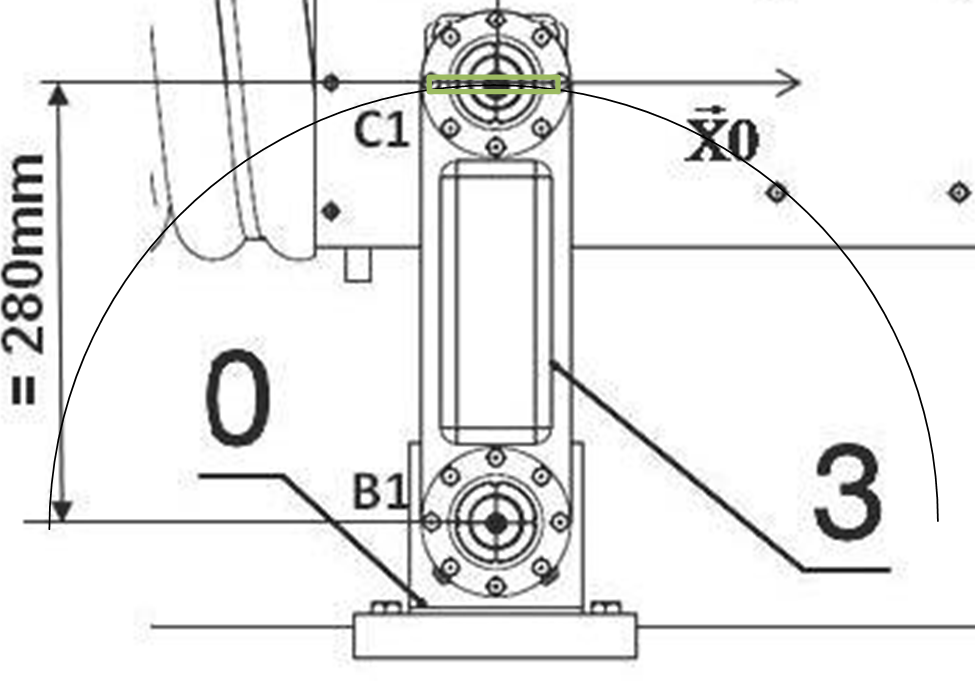
\includegraphics[width=0.3\linewidth]{img/trajectoire}
\end{center}

\paragraph{Question 4:} $\delta=R-R\sqrt{R^2-\delta^2}=0,8mm$.

\paragraph{Question 5:} Le ration est de $\frac{0,8}{40}=0,02$.

\paragraph{Question 6:} $\overrightarrow{AF}+\overrightarrow{FG}+\overrightarrow{GH}+\overrightarrow{HA}=\overrightarrow{0}$

Sur $\overrightarrow{x_0}$: $-e.sin\theta(t)-R+x_H=0$, donc $x_H=R+e.sin\theta(t)$.

\paragraph{Question 7:} $\overrightarrow{V_{H\in7/R0}}=\frac{dx_H}{dt}.\overrightarrow{x_0}$, avec $\frac{dx_H}{dt}=-e.\dot{\theta}.cos\theta(t)$.

\paragraph{Question 8:} 

\begin{center}
 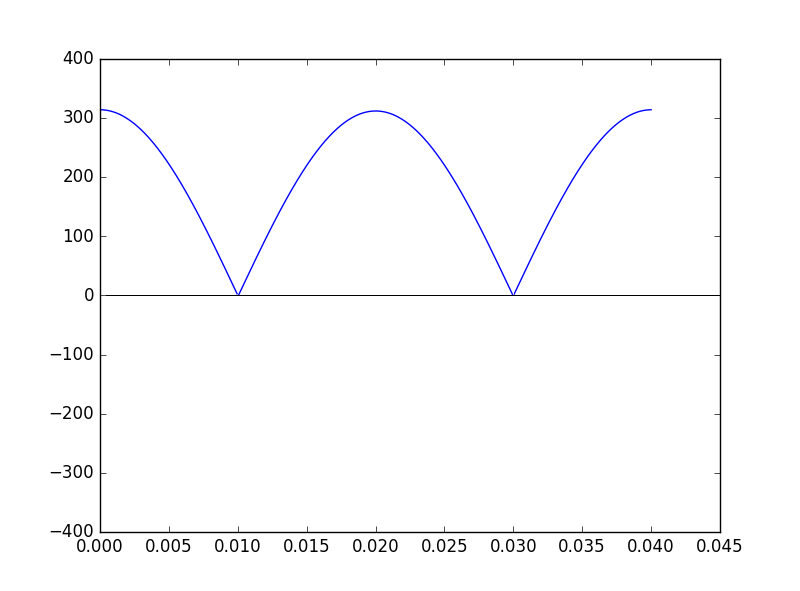
\includegraphics[width=0.7\linewidth]{img/figure_3}
\end{center}

\subsection{Banc d'épreuve hydraulique}

\paragraph{Question 1:} $h=R.cos 35=328mm$, $c=2.R.sin35=459mm$.

\paragraph{Question 2:} $\overrightarrow{V_{A\in1/0}}=R.\dot{\theta}.\overrightarrow{x_1}$.

$\overrightarrow{V_{A\in1/0}}=\overrightarrow{V_{A\in1/2}}+\overrightarrow{V_{A\in2/3}}+\overrightarrow{V_{A\in3/0}}$

$\overrightarrow{V_{A\in1/0}}=\dot{x}.\overrightarrow{x_2}+x.\dot{\varphi}.\overrightarrow{y_2}$

Donc, $tan\varphi=\frac{\dot{x}.cos\varphi-R.\dot{\theta}.cos\theta}{R.\dot{\theta}.sin\theta-\dot{x}.sin\varphi}$

Donc, $\dot{\theta}=\frac{\dot{x}}{R.cos(\theta_1-\varphi)}$

\subsection{Chaudière à bois déchiqueté}
 
\paragraph{Question 1:} $\overrightarrow{OA}+\overrightarrow{AB}+\overrightarrow{BC}+\overrightarrow{CO}=\overrightarrow{0}$
 
$\left\{\begin{array}{l}
r.cos\theta_{10}-l.sin\theta_{20}-R.cos\theta_{30}+L=0 \\
r.sin\theta_{10}-l.cos\theta_{20}-R.sin\theta_{30}=0
\end{array}\right.$

$r^2+R^2+L^2-2.r.R.cos\theta_{10}.cos\theta_{30}+2.L.(r.cos\theta_{10}-R.cos\theta_{30})-2.R.r.sin\theta_{10}.sin\theta_{30}=l^2$

\paragraph{Question 2:} Il faudrait dériver ce résultat.

\paragraph{Question 3:} $\overrightarrow{V_{D\in 3/0}}=\overrightarrow{V_{C\in 3/0}}+\overrightarrow{DC}\wedge \overrightarrow{\Omega_{3/0}}$

$\overrightarrow{V_{D\in 3/0}}=d.\omega_{30}.\overrightarrow{y_3}^*$

avec $\overrightarrow{y_3}^*=-sin(\theta_{30}+\alpha).\overrightarrow{x_0}+cos(\theta_{30}+\alpha).\overrightarrow{x_0}$,

Donc, $\overrightarrow{V_{D\in 3/0}}=d.\omega_{30}.(-sin(\theta_{30}+\alpha).\overrightarrow{x_0}+cos(\theta_{30}+\alpha).\overrightarrow{y_0})$

\paragraph{Question 4 et 5:}

\begin{center}
 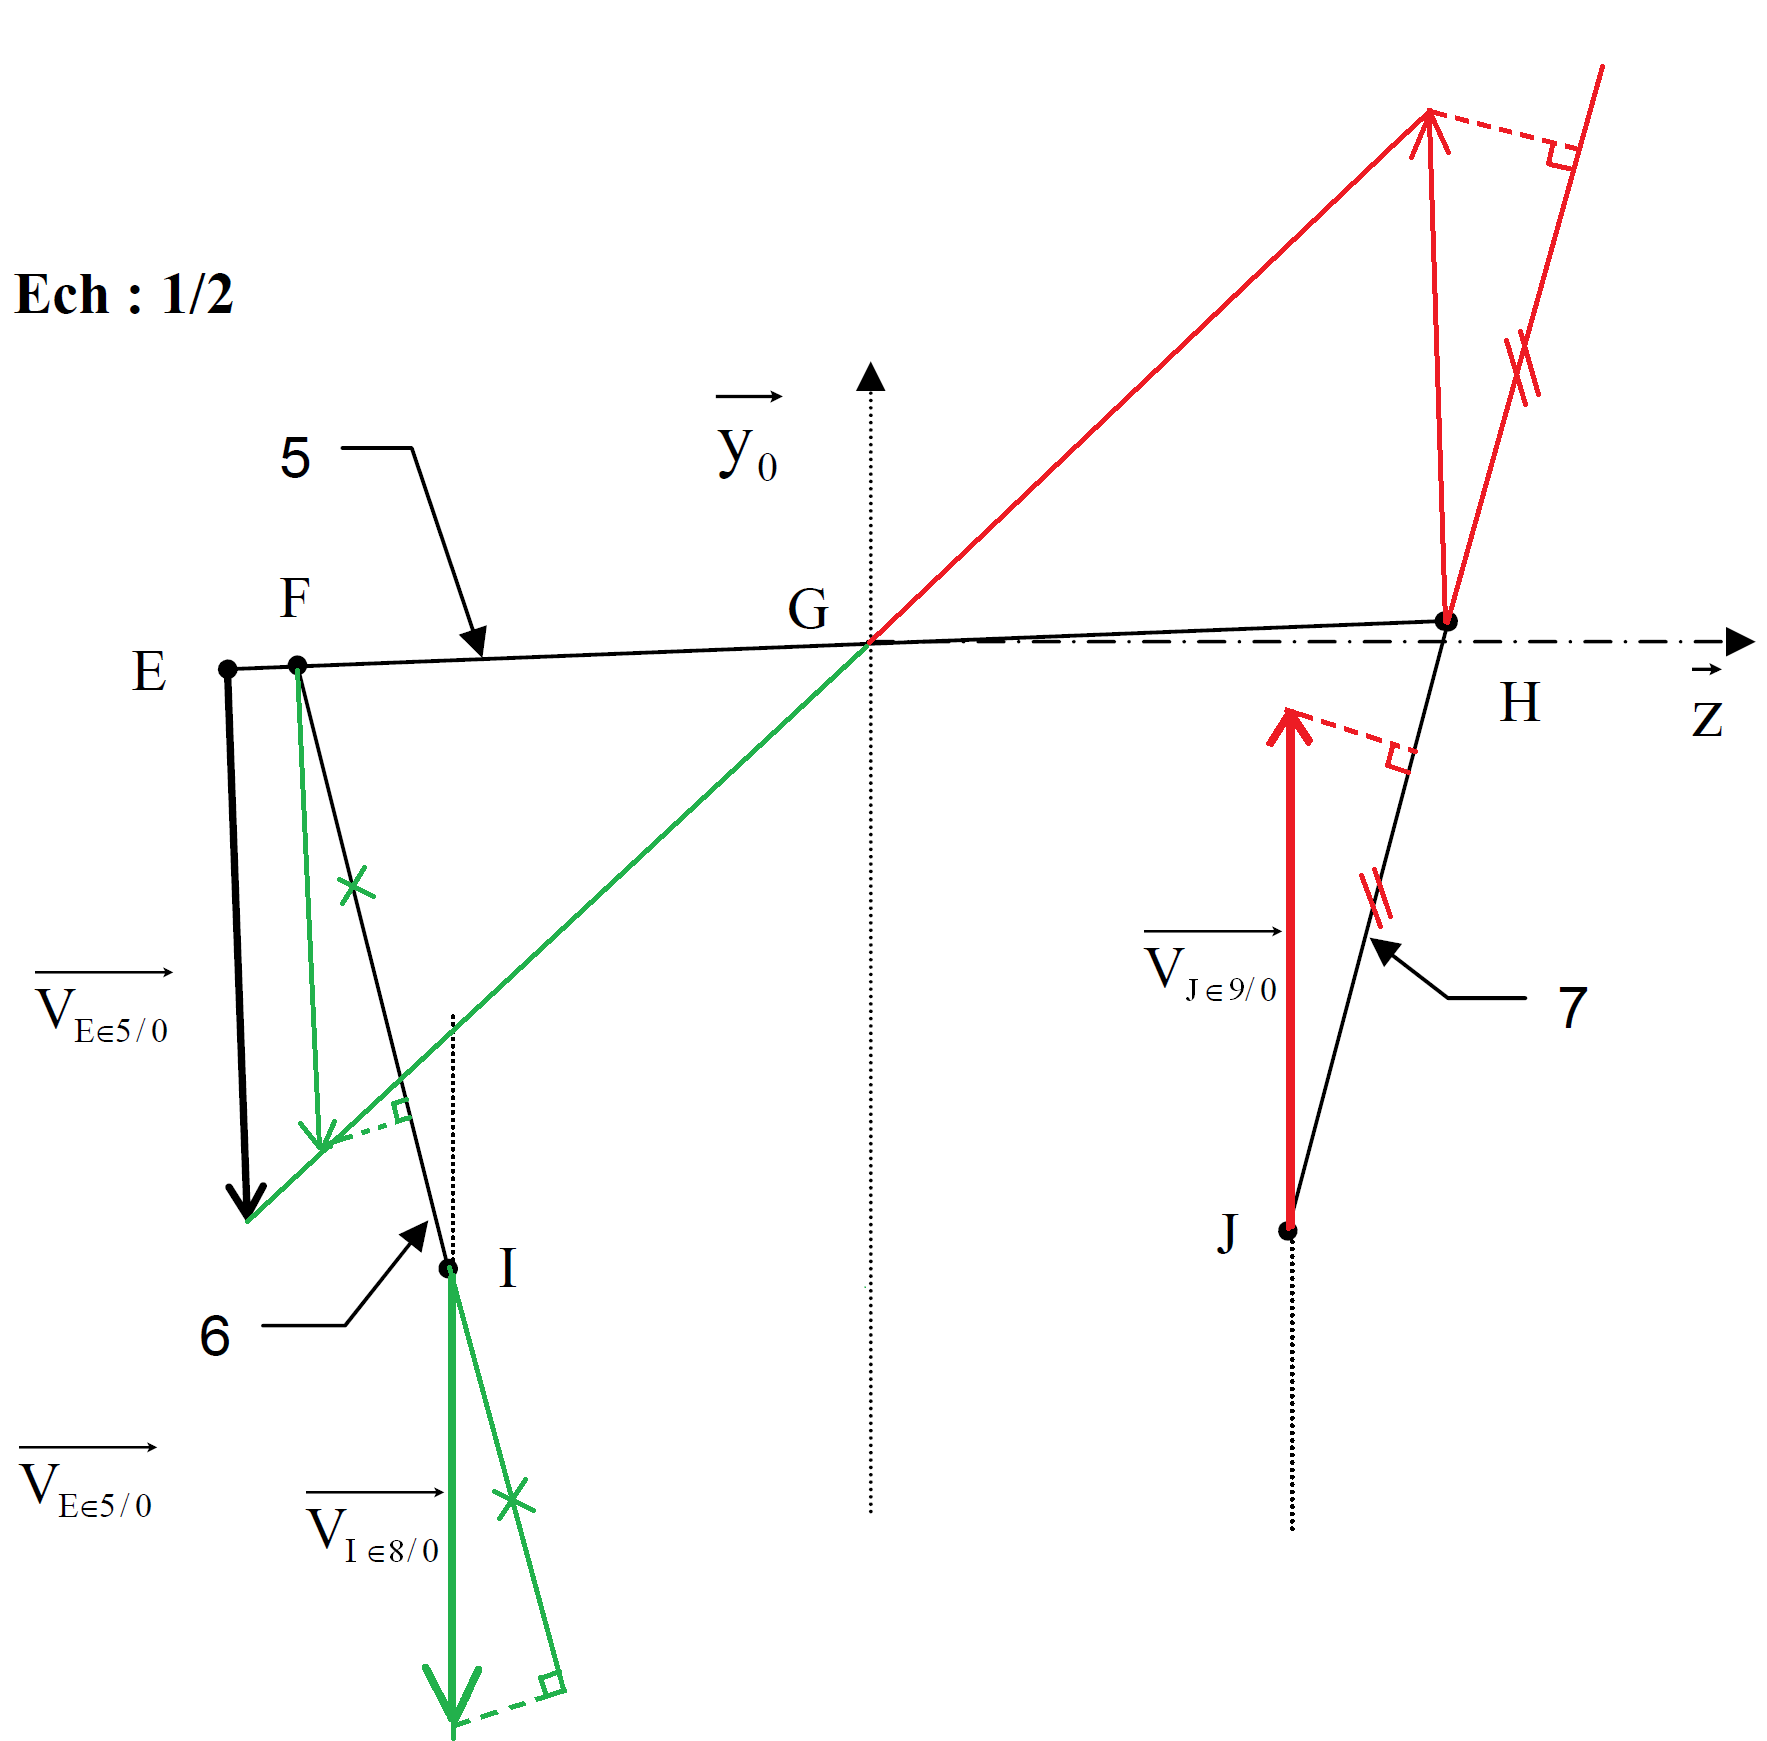
\includegraphics[width=0.8\linewidth]{img/chaudiere_cin_graph_cor}
\end{center}

\paragraph{Question 6:}

\begin{center}
 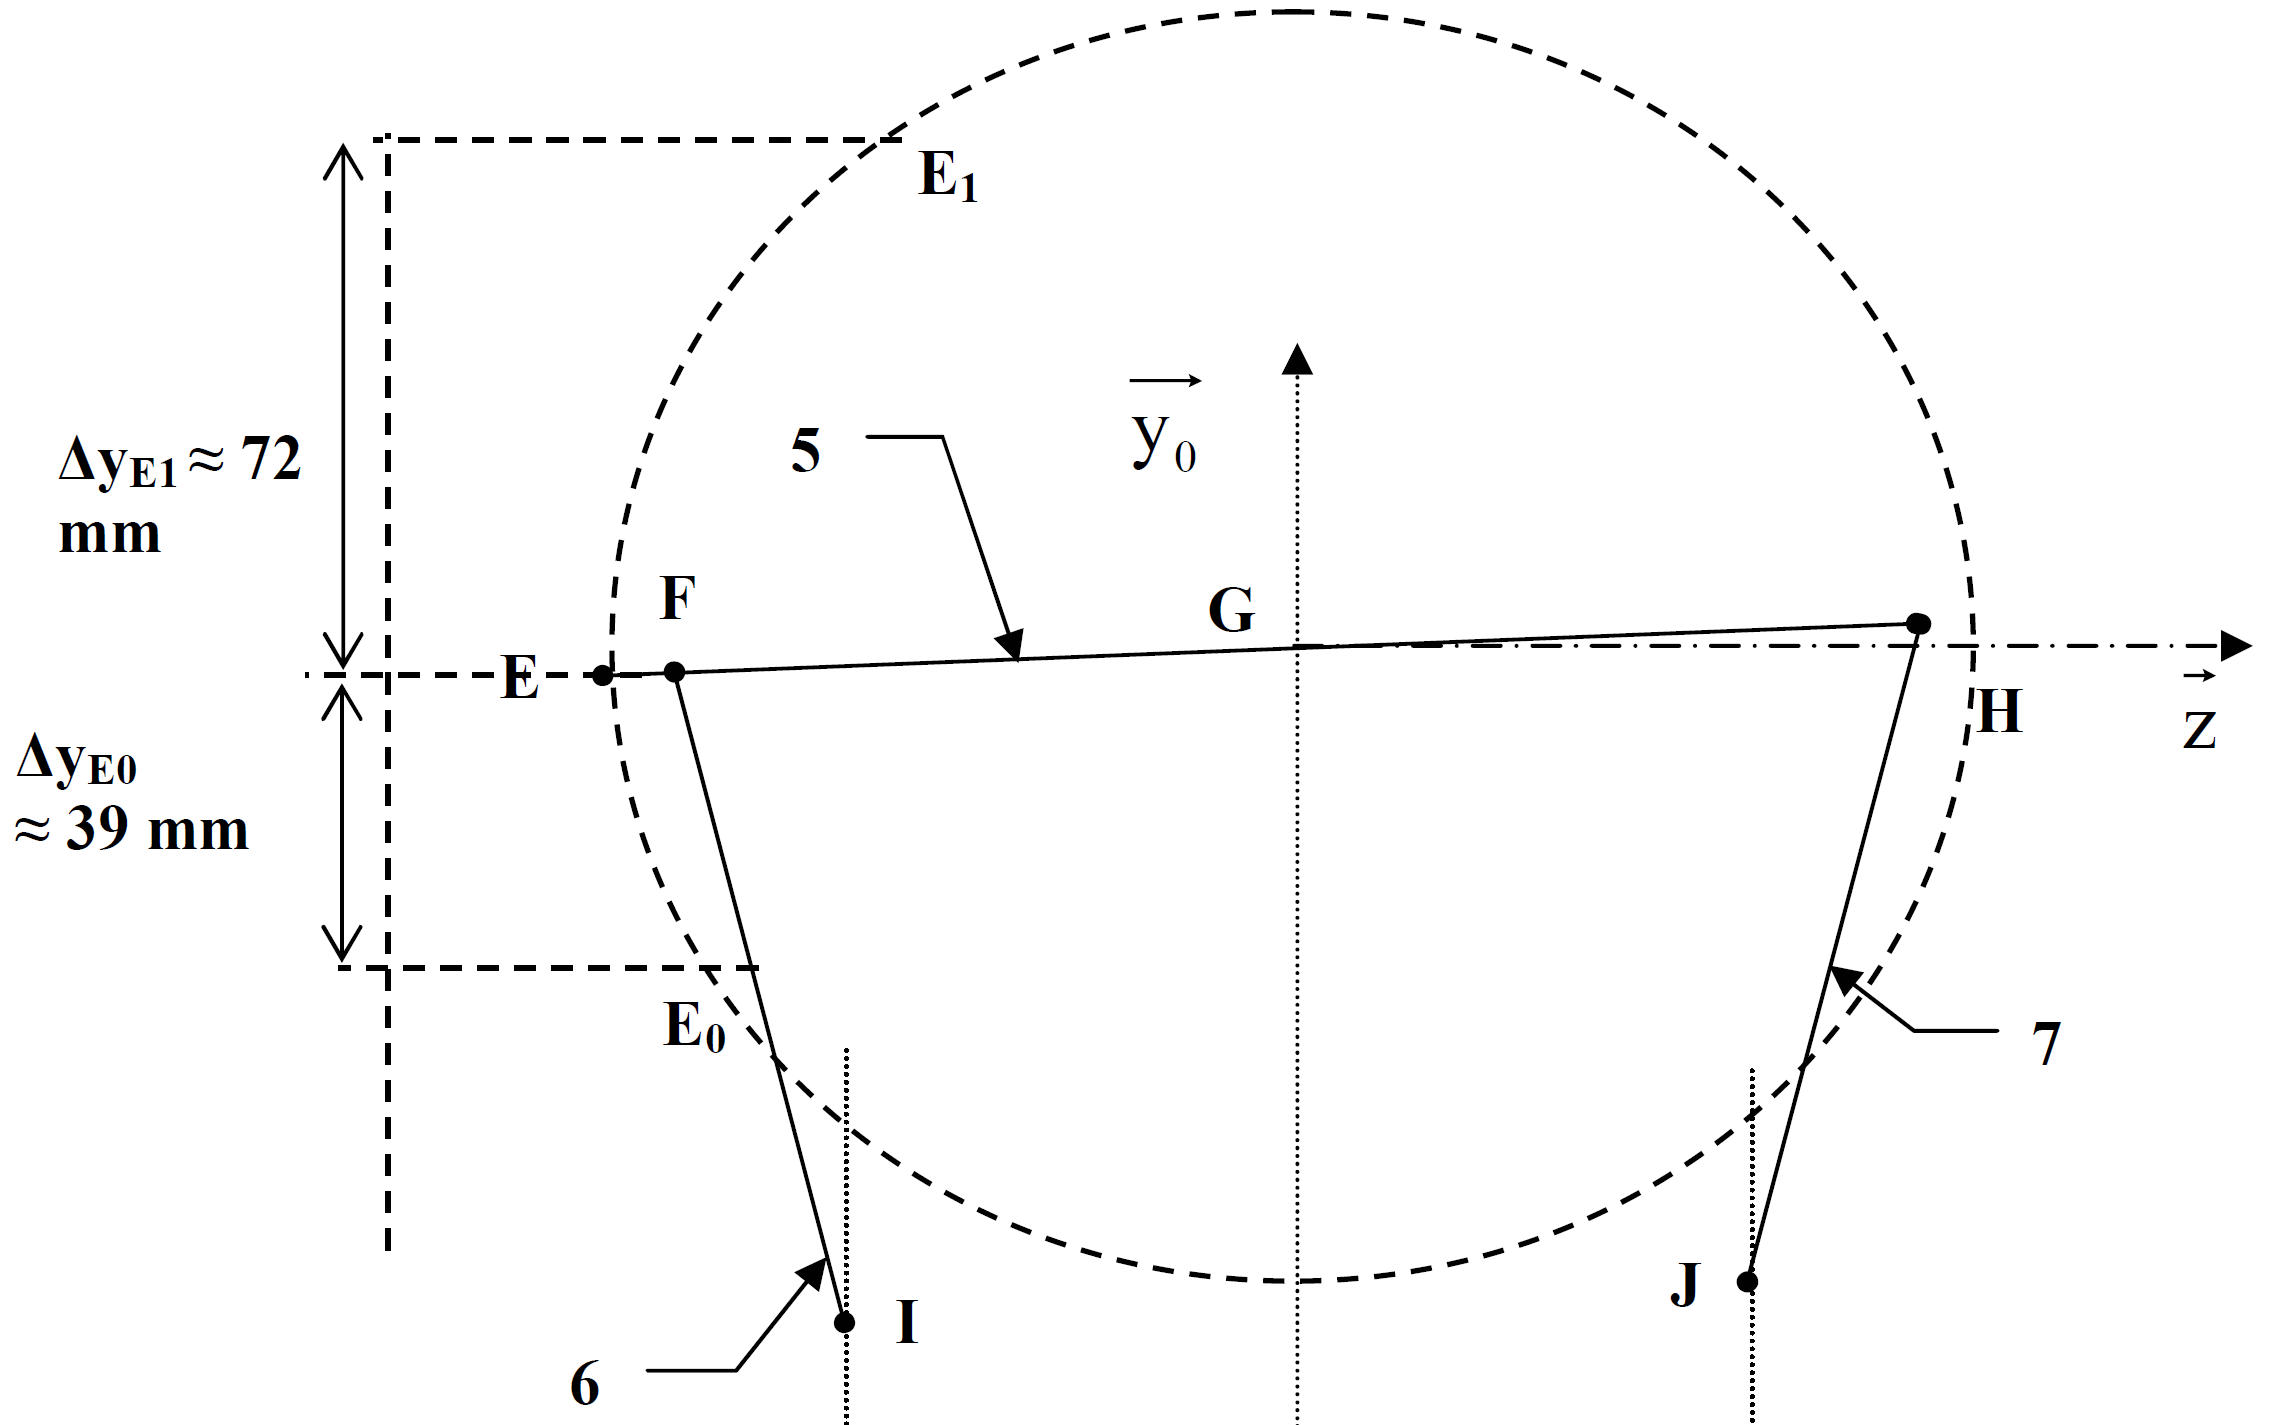
\includegraphics[width=0.8\linewidth]{img/chaudiere_geom_cor_2}
\end{center}

\paragraph{Question 7:}

Le point D se déplace d'environ 45 mm suivant $\overrightarrow{x_0}$ ce qui peut être négligé devant la longueur de la tringle de 1150 mm. Ce mouvement peut donc être considéré comme un mouvement de translation de direction $\overrightarrow{y_0}$.


\paragraph{Question 8:}

\begin{center}
 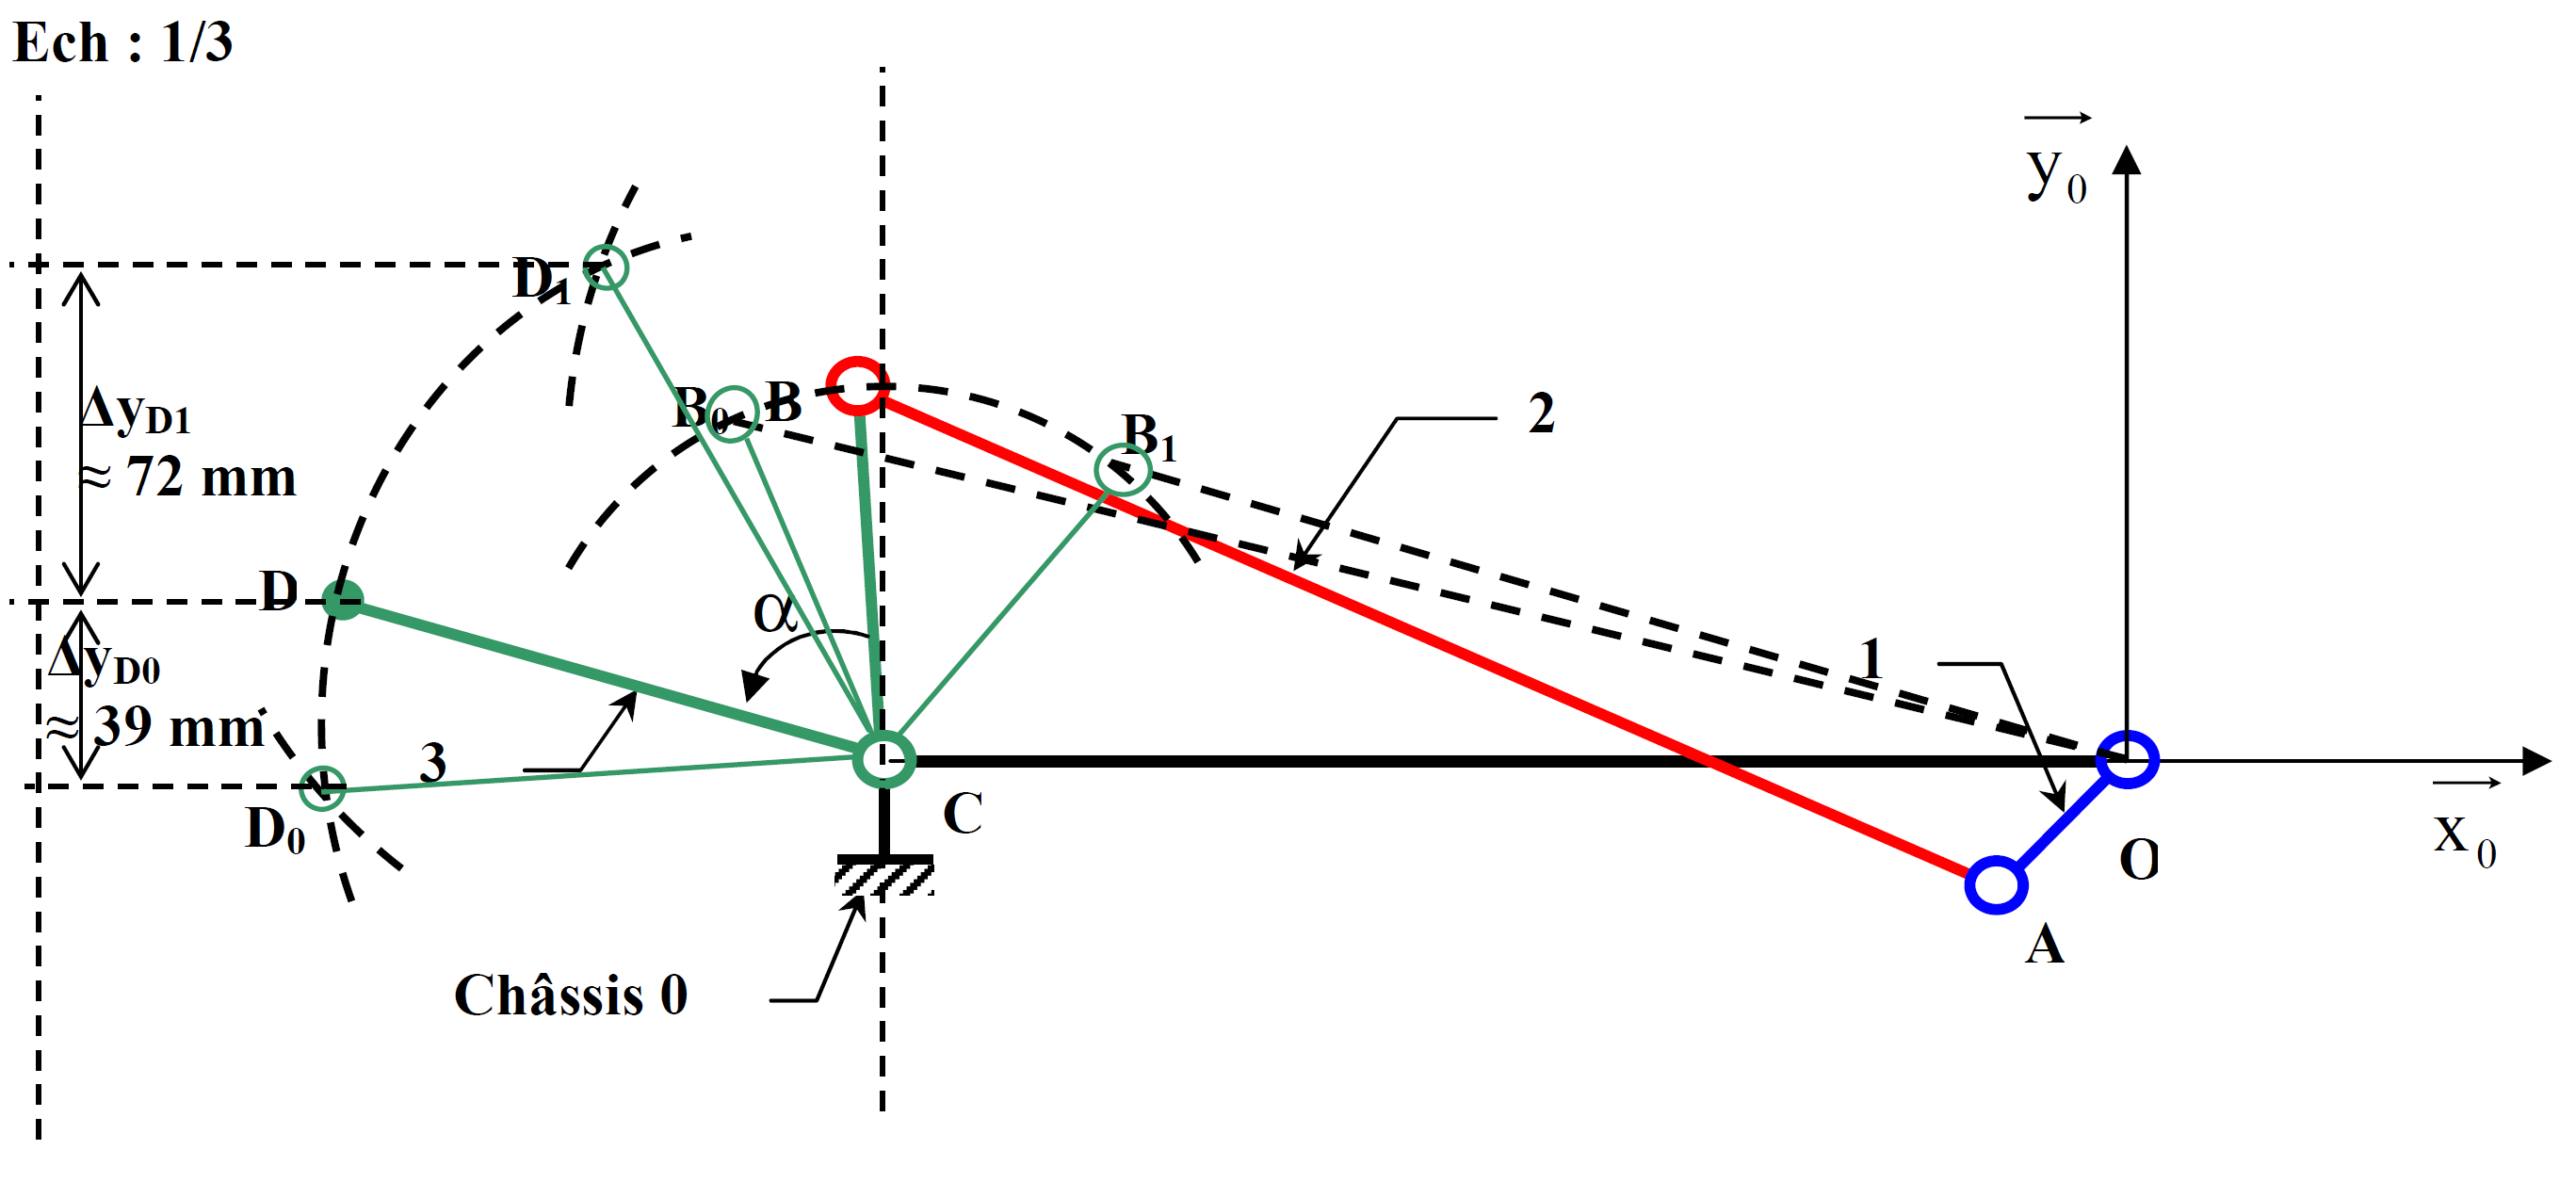
\includegraphics[width=0.8\linewidth]{img/chaudiere_geom_cor}
\end{center}


\paragraph{Question 9:}

$\overrightarrow{V_{D\in4/0}}=\overrightarrow{V_{D\in3/0}}=d.\omega_{30}.cos(\alpha+\theta_{30}).\overrightarrow{y_0}$

Donc $V_{40}=d.K_1.\omega_{10}.cos(\alpha+\theta_{30})$ avec $\alpha+\theta_{30}=95+70=165\degree$

Or $cos(165\degree)\approx -1$ donc : $V_{40}=-d.K_1.\omega_{10}$

\paragraph{Question 10:}

Dans la position donnée : $V_{E50}\approx V_{40}$ et $\omega_{10}=4rad.s^{-1}$

Donc

$\||V_{80}\||=\||K_{85}.V_{E50}\||=\||K_{85}.V_{40}\||=\frac{35}{40}.\frac{1}{2}.4.0,12\approx 0,21m.s^{-1}$

$\||V_{90}\||=\||K_{95}.V_{E50}\||=\||K_{95}.V_{40}\||=\frac{33}{40}.\frac{1}{2}.4.0,12\approx 0,19m.s^{-1}$

La vitesse des turbulateurs par rapport à l'échangeur est donc bien comprise entre $0,15$ et $0,25m.s^{-1}$

\subsection{Mécanisme de commande de pompe doseuse}

\paragraph{Question 1:} $course=2.e$ donc $course=30mm$.

\paragraph{Question 2:} $c=2e.\frac{\lambda cos\gamma_0}{d-\lambda cos\gamma_0}$

Applications numériques :
\begin{itemize}
	\item $\lambda = 30 mm : c = 9,48mm$,
	\item $\lambda = 45 mm : c = 16,9 mm$,
	\item $\lambda = 60 mm : c = 27,7 mm$. 
\end{itemize}

\paragraph{Question 3:} $\overrightarrow{AB}+\overrightarrow{BC}+\overrightarrow{CA}=\overrightarrow{0}$

$x=e cos\alpha + \sqrt{L^2-e^2 sin^2 \alpha}$ et $sin\beta = -\frac{e.sin\alpha}{L}$.

\paragraph{Question 4:} $(\overrightarrow{AC_1}+\overrightarrow{C_1D}).\overrightarrow{x_0}=(\overrightarrow{AC}+\overrightarrow{CD}).\overrightarrow{x_0}$

$tan\gamma=\frac{e+L+d.tan\gamma_0-\lambda sin\gamma_0 -x}{d-\lambda cos\gamma_0}$

\paragraph{Question 5:} 

\begin{center}
 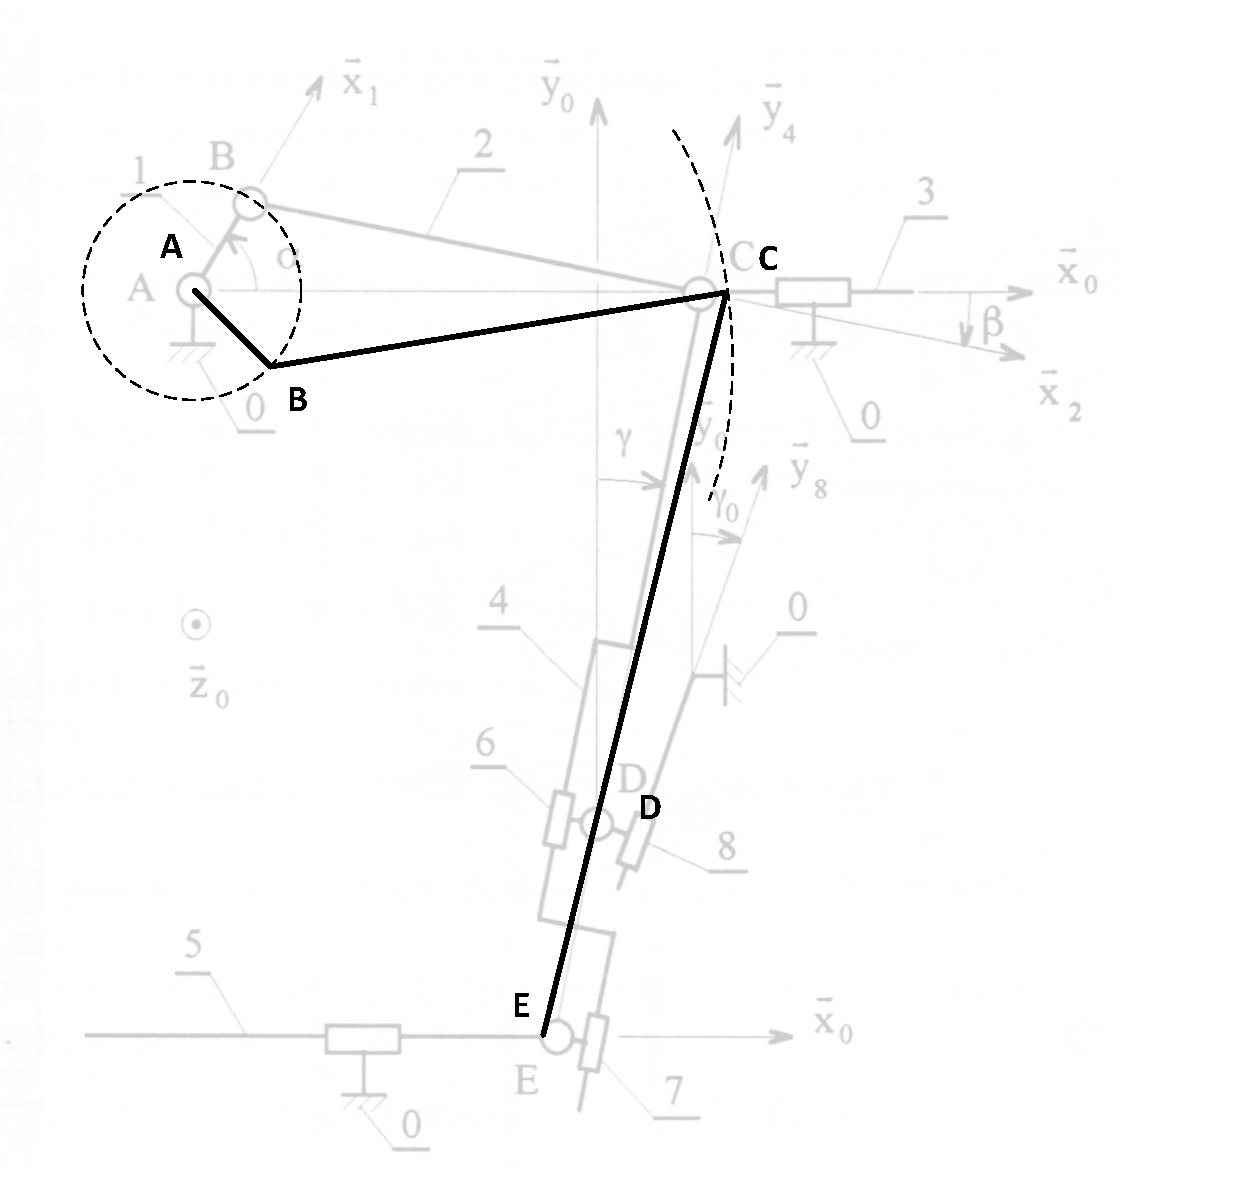
\includegraphics[width=0.8\linewidth]{img/epure_cor}
\end{center}

\paragraph{Question 6:} 

\begin{center}
 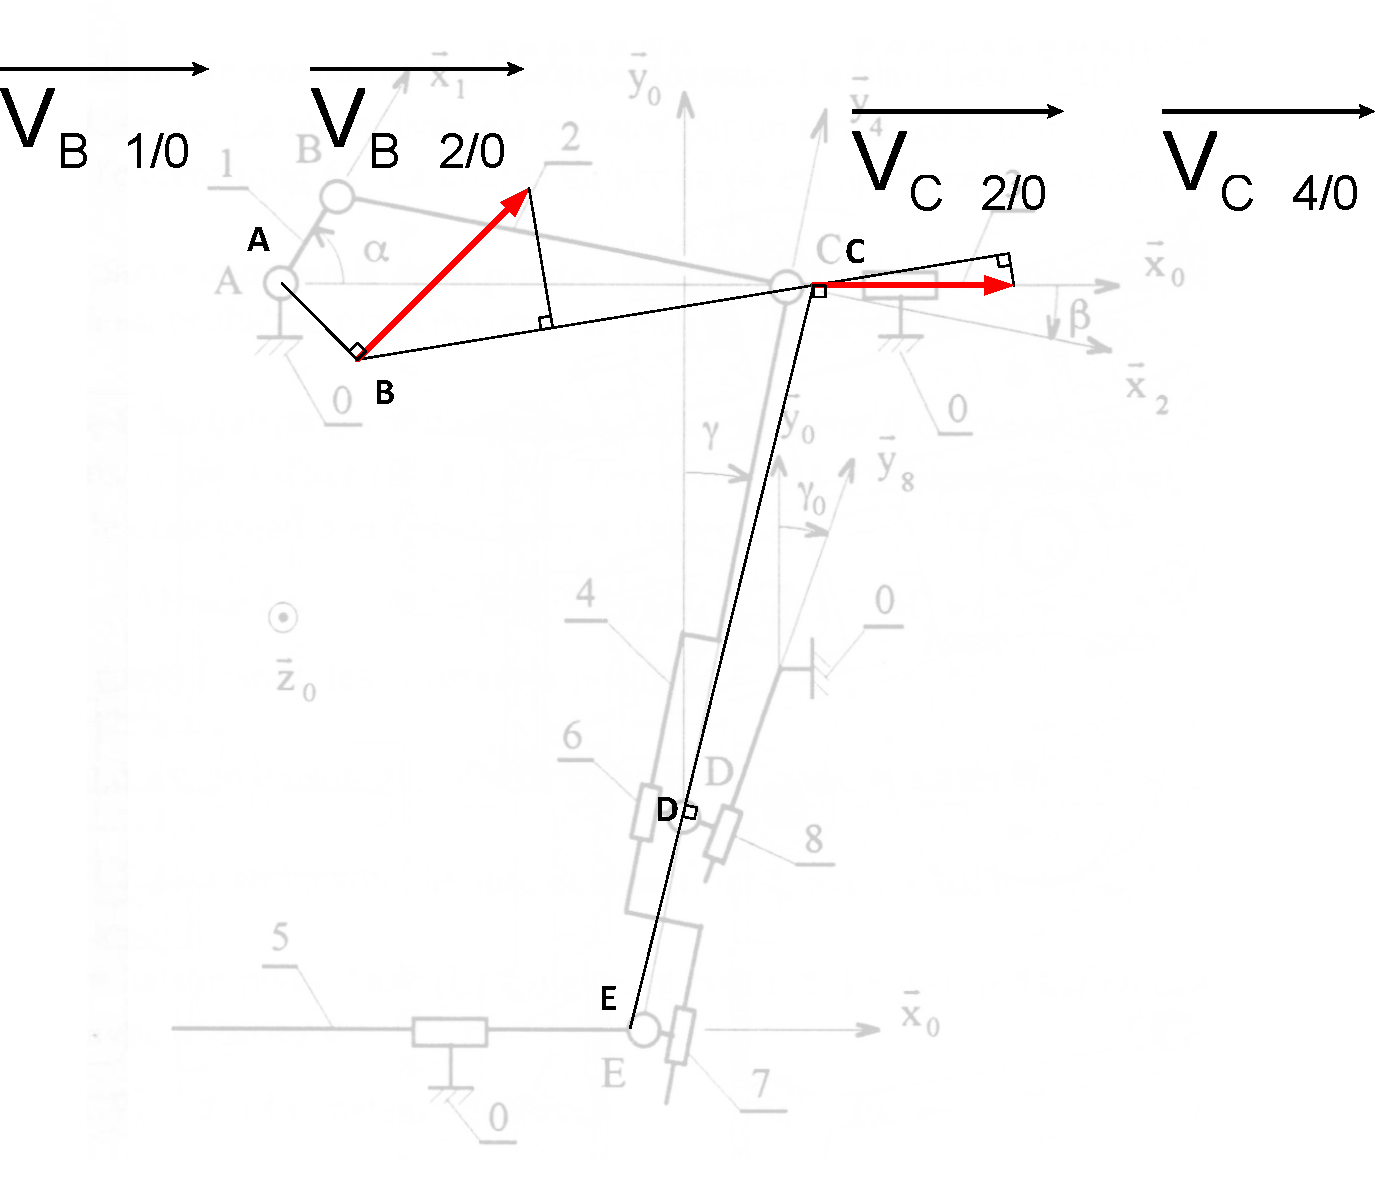
\includegraphics[width=0.8\linewidth]{img/reglage_cor_cin_1}
\end{center}

\begin{center}
 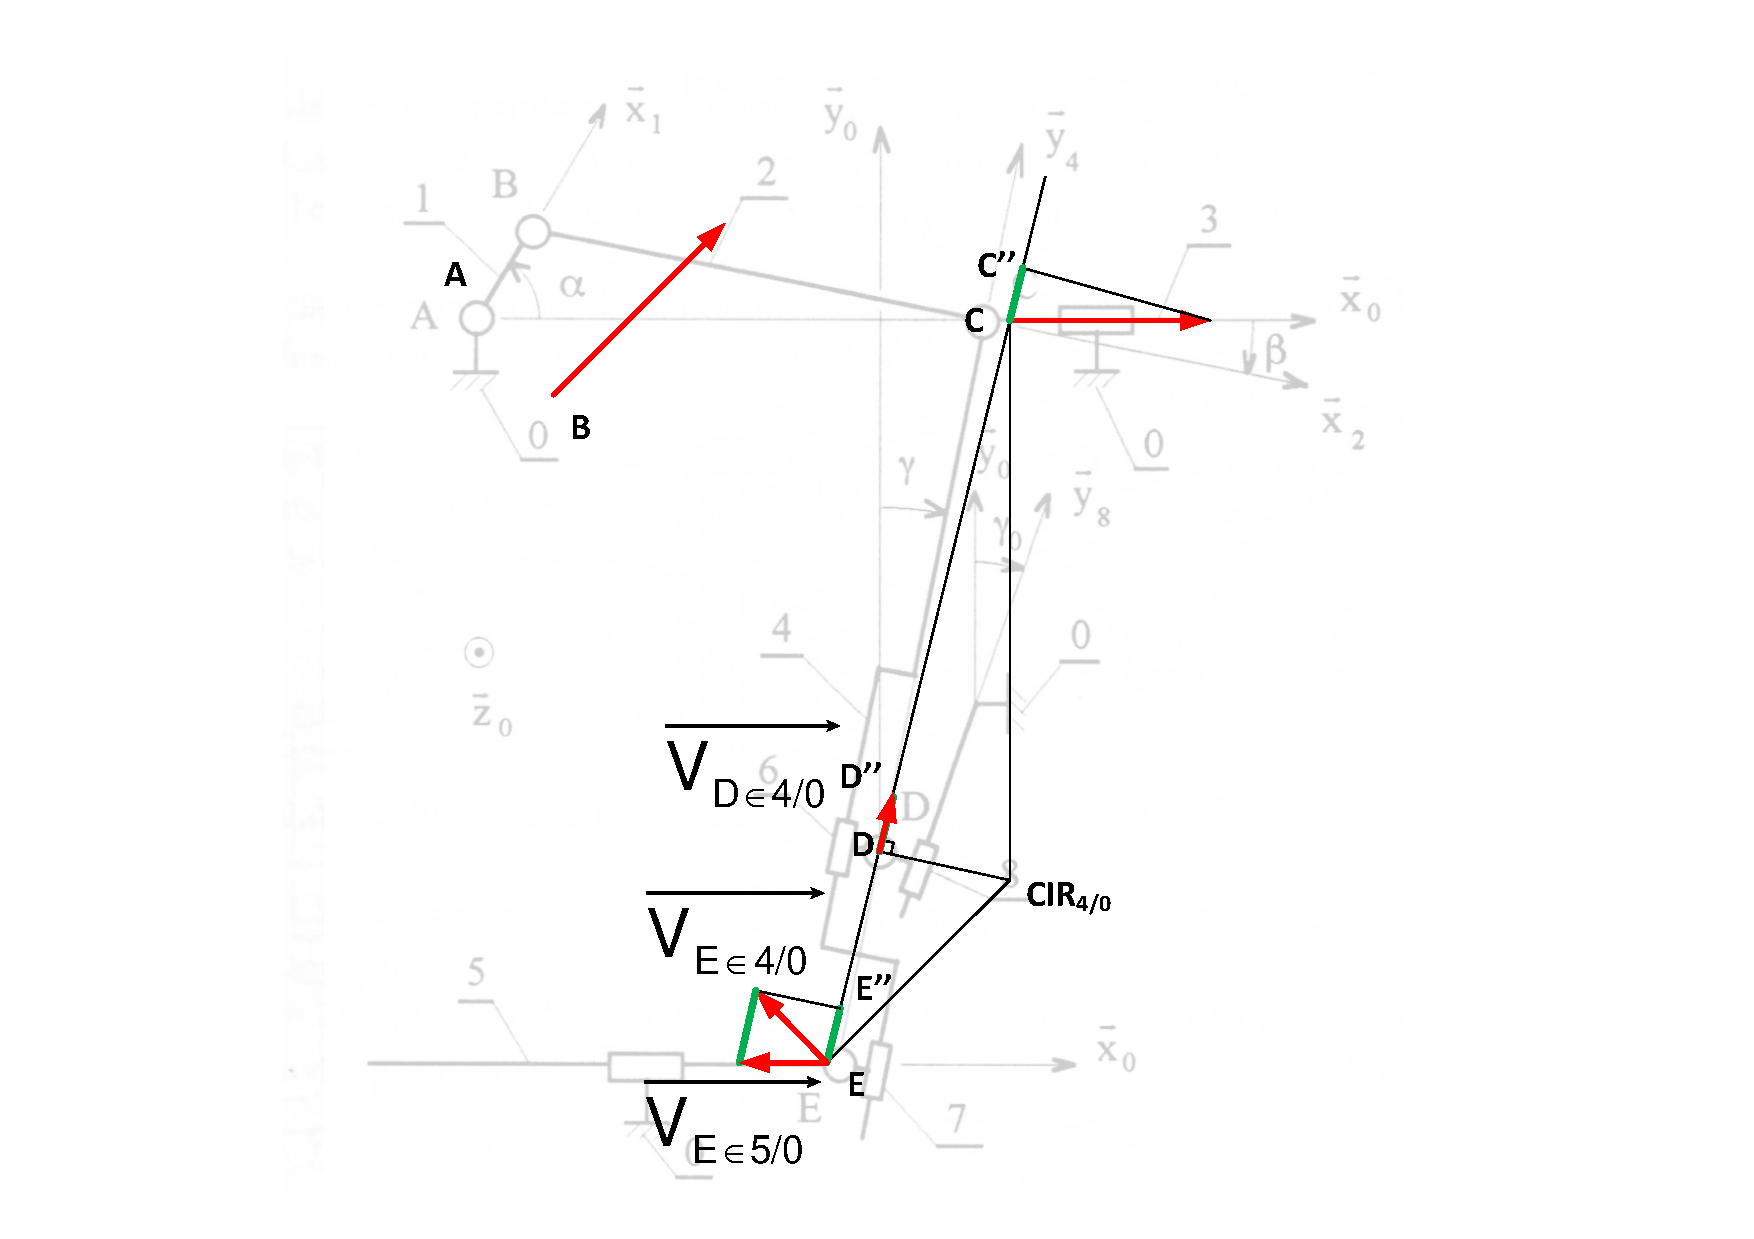
\includegraphics[width=0.8\linewidth]{img/reglage_cor_cin_2}
\end{center}

\paragraph{Question 7:} 

$\overrightarrow{V_{E\in5/0}}=\left[\frac{d}{dt}\overrightarrow{AE}\right]_0=\left[\frac{d}{dt}\overrightarrow{E_1E}\right]_0$

On a : $\frac{E_1E}{CC_1}=\frac{E_1D}{DC_1}$

On a : $\frac{E_1E}{e+L-x}=\frac{\lambda}{\frac{d}{cos\gamma_0}-\lambda}$, donc $\overrightarrow{E_1E}=(e+L-x).\frac{\lambda}{d-\lambda.cos\gamma_0}.\overrightarrow{x_0}$,

donc $\overrightarrow{V_{E\in5/0}}=-\dot{x}.\frac{\lambda.cos\gamma_0}{d-\lambda.cos\gamma_0}.\overrightarrow{x_0}$

\paragraph{Question 8:}

$\overrightarrow{V_{D\in 4/6}}=\overrightarrow{V_{D\in 4/0}}+\overrightarrow{V_{D\in 6/0}}$

$\overrightarrow{V_{D\in 4/6}}=-\dot{x}.sin\gamma.\overrightarrow{y_4}$

\paragraph{Question 9.a:}

$\overrightarrow{V_{E\in 4/7}}=\overrightarrow{V_{E\in 4/0}}-\overrightarrow{V_{D\in 7/0}}$

$\overrightarrow{V_{C\in 4/0}}.\overrightarrow{y_4}=\overrightarrow{V_{C\in 2/0}}.\overrightarrow{y_4}=-\dot{x}.sin\gamma$

$\overrightarrow{V_{E\in 5/0}}.\overrightarrow{y_4}=-\dot{x}.\frac{\lambda.cos\gamma_0}{d-\lambda.cos\gamma_0}.sin\gamma$

Donc, $\overrightarrow{V_{E\in 4/7}}=-\dot{x}.\frac{d}{d-\lambda.cos\gamma_0}.sin\gamma.\overrightarrow{y_4}$

\paragraph{Question 9.b:}

Le graphe de $\overrightarrow{V_{E\in 4/7}}$ est le même que le graphe $\overrightarrow{V_{D\in 4/6}}$ à un coefficient multiplicateur près:
\begin{itemize}
 \item $\lambda=30mm$: $1,32$,
 \item $\lambda=45mm$: $1,56$,
 \item $\lambda=60mm$: $1,92$.
\end{itemize}

\paragraph{Question 9.c:}

Max de $V_{E\in4/7}$:
\begin{itemize}
 \item $\lambda=30mm$: $0,08m.s^{-1}$,
 \item $\lambda=45mm$: $0,1m.s^{-1}$,
 \item $\lambda=60mm$: $0,13m.s^{-1}$.
\end{itemize}
\paragraph{Question 10:}

$\overrightarrow{\Omega_{2/1}}=\overrightarrow{\Omega_{2/0}}-\overrightarrow{\Omega_{1/0}}=(\dot{beta}-\dot{\alpha}).\overrightarrow{z_0}$

En sachant, $e.sin\alpha+L.sin\beta=0$, d'où $e.cos\alpha.\dot{\alpha}+L.cos\beta.\dot{\beta}=0$

On obtient: $\dot{\beta}=-\frac{e.cos\alpha}{\sqrt{L^2-e^2.sin^2\alpha}}.\dot{\alpha}$

Ainsi, $\overrightarrow{\Omega_{2/1}}=-\left(1+\frac{e.cos\alpha}{\sqrt{L^2-e^2.sin^2\alpha}}\right).\dot{\alpha}.\overrightarrow{z_0}$

\end{document}
